% !TEX TS-program = pdflatex
% !TEX encoding = UTF-8 Unicode


\documentclass[12pt,final,oneside]{dwThesis} % use larger type; default would be 10pt

\usepackage[utf8]{inputenc} % set input encoding (not needed with XeLaTeX)
\usepackage[margin=2cm]{geometry}
\usepackage{xy}
\usepackage{amsmath, amsthm}
\usepackage{showkeys}
%\usepackage[smaller]{acronym}
%\usepackage{natbib}
\usepackage{tabularx}
\newcolumntype{R}{>{\raggedleft\arraybackslash}X}
\usepackage{chngpage}
\usepackage{booktabs}
\usepackage{cite}
\usepackage{times}
\usepackage{graphicx}
\usepackage{ctable}
\usepackage{footnote}
\usepackage{amssymb}
\usepackage{url}
\usepackage{placeins}
\usepackage{tameflts}
\usepackage{algpseudocode}
\usepackage{cite}
\usepackage{algorithm}
\usepackage{eqparbox,array}
\renewcommand\algorithmiccomment[1]{%
  \hfill$\triangleright$\ \parbox[t]{.25\linewidth}{#1}%
}
\algrenewcommand\Return{\State \algorithmicreturn{} }%
\usepackage{tikz-timing}
\usepackage[lofdepth,lotdepth]{subfig}
\usepackage{multirow}
\usepackage{tameflts}
\usepackage[bookmarks,hidelinks]{hyperref}
\usepackage[nonumberlist]{glossaries}
\usepackage[inline,index]{fixme}
\makeglossaries
\fxsetup{
   status=draft,
   author=,
   layout={inline,index,marginclue}, % also try footnote or pdfnote
   theme=color
}
\definecolor{fxnote}{rgb}{0.8000,0.0000,0.0000}

\OnehalfSpacing
\setcounter{tocdepth}{3}

\usepackage{color}
\usepackage{listings}
\lstset{ %
   language=C++,                % choose the language of the code
   basicstyle=\ttfamily,       % the size of the fonts that are used for the code
   numbers=left,                   % where to put the line-numbers
   numberstyle=\footnotesize,      % the size of the fonts that are used for the line-numbers
   stepnumber=1,                   % the step between two line-numbers. If it is 1 each line will be numbered
   numbersep=5pt,                  % how far the line-numbers are from the code
   backgroundcolor=\color{white},  % choose the background color. You must add \usepackage{color}
   showspaces=false,               % show spaces adding particular underscores
   showstringspaces=false,         % underline spaces within strings
   showtabs=false,                 % show tabs within strings adding particular underscores
   frame=single,           % adds a frame around the code
   tabsize=2,          % sets default tabsize to 2 spaces
   captionpos=b,           % sets the caption-position to bottom
   breaklines=false,        % sets automatic line breaking
   breakatwhitespace=false,    % sets if automatic breaks should only happen at whitespace
   escapeinside={\%*}{*)}          % if you want to add a comment within your code
}

%%% END Article customizations

%%% The "real" document content comes below...
\setlength\overfullrule{0pt}
\title{VPR Assessment of a Novel Partitioning Algorithm}
\author{David Munro}
\studentnumber{z3218420}
\collegeordept{School of Computer Science and Engineering}
\university{The University of New South Wales}
\degree{Bachelor of Engineering (Computer)}
\degreedate{June, 2013}
\supervisor{Oliver Diessel}
\assessor{Sri Parameswaran}
%\date{} % Activate to display a given date or no date (if empty),
% otherwise the current date is printed

\newacronym{VPR}{VPR}{Versatile Place and Route}
\newacronym{MCNC}{MCNC}{Microelectronics Centre of North Carolina}
\newacronym{BLE}{BLE}{Basic Logic Element}
\newacronym{CLB}{CLB}{Configurable Logic Block}
\newacronym{DFG}{DFG}{Directed Flow Graph or Data Flow Graph}
\newacronym{DAG}{DAG}{Directed Acyclic Graph}
\newacronym{SEU}{SEU}{Single Event Upset}
\newacronym{LUT}{LUT}{Lookup Table}
\newacronym{VTR}{VTR}{Verilog To Routing Project}
\newacronym{ABC}{ABC}{A System for Sequential Synthesis and Verification}
\newacronym{FPGA}{FPGA}{Field-Programmable Gate Array}
\newacronym{TMR}{TMR}{Triple Modular Redundancy}
\newacronym{BLIF}{BLIF}{Berkeley Logic Interchange Format}
\newacronym{ASIC}{ASIC}{Application-Specific Integrated Circuit}
\newacronym{LAB}{LAB}{Logic Array Block}
\newacronym{IO}{IO}{Input/Output}
\newacronym{ICAP}{ICAP}{Internal Configuration Access Port}
\newacronym{SRAM}{SRAM}{Static RAM}
\newacronym{mux}{mux}{Multiplexer}
\newacronym{CAD}{CAD}{Computer-Aided Design}
\newacronym{MBU}{MBU}{Multi-Bit Upset}
\newacronym{NRE}{NRE}{Non-Recurring Engineering}
\newacronym{DICE}{DICE}{Dual Interlock Storage Cell}
\newacronym{VHDL}{VHDL}{VHSIC Hardware Description Language}
\newacronym{SAT}{SAT}{Boolean Satisfiability Problem}
\newacronym{CPU}{CPU}{Central Processing Unit}

\newglossaryentry{primitive}{name=primitive,
   description={Most basic circuit element. Either a latch or a \gls{LUT}},
   first=\textit{primitive}
}
\newglossaryentry{scrubbing}{name=scrubbing,
   description={Refreshing an \gls{FPGA}'s configuration memory to purge accumulated erorrs },
   first=\textit{scrubbing}
}

\begin{document}

 \pagenumbering{roman}
   \maketitle
   \fxfatal{Need to fix title to match CSE requirements, and check other format restrictions}

   \begin{acknowledgements}
      I would like to thank my supervisor Oliver Diessel
      for his assistance and advice throughout the entire process. I also wish
      to thank Patricia Munro, Salima Yeung, Michelle Kopack and  for their proofreading.


   \end{acknowledgements}

   \begin{abstracts}
      \gls{FPGA} systems would be well
      suited to space-based applications except for their vulnerability to
      space-based radiation. Various techniques for dealing with their
      susceptibility have been discussed in the literature.
      A key part of a theoretical technique to protect against radiation-induced \glspl{SEU}
      was developed and the implementation assessed using open-source tools.
      Results indicate that the developed algorithm exhibited respectable performance compared
      to existing alternatives while providing theoretically greater fault tolerance, although further work is required to implement 
      the algorithm for current commercial devices.
      
      
      %This thesis aims to
      %develop and assess a key part of a theoretical technique to protect
      %against radiation-induced \glspl{SEU} and to assess the overheads of the
      %technique.  \glsresetall 
   \end{abstracts}
   \newpage \tableofcontents*
   \listoftables
   \listoffigures
   \fxerror{Fix formatting on ToC}
   \listoffixmes \newpage \printglossaries 

   \glsresetall
   \glsunset{VHDL} 
   \glsunset{ABC} 
   \glsunset{CPU}
   \chapter{Introduction}
   \pagenumbering{arabic} 
   \section{Overview}
   Space plays an increasingly
   important role in the functioning of modern societies, being vital for
   fields including navigation, meteorology, and
   communications\cite{OECDSpace}. \gls{FPGA} systems have many beneficial
   features, such as their flexibility and low \gls{NRE} costs which make them
   highly desirable for space-based applications. Unfortunately they have far
   greater susceptibility to space radiation. Hardened \glspl{FPGA} offer only
   a fraction of the gate counts (and hence capability of implementing large or
   complex circuits) of non-hardened offerings prompting a search for a
   solution to the radiation susceptibility of \glspl{FPGA} using mainstream
   hardware, one of the most popular of which is \gls{TMR}\cite{VFPGATMR}. In
   \gls{TMR}, vulnerable components are triplicated allowing for errors to be
   detected and mitigated. This thesis is based on the work
   of\cite{DiesselChange} which introduces an approach to \gls{TMR}, and aims
   to develop a key part of the approach and assess the implementation with the
   aid of an open-source \gls{CAD} toolchain for \glspl{FPGA}.
   
   The remainder of this chapter provides an overview of
   these technologies, discusses alternatives to our approach, and details why
   we have chosen the technique we have. Chapter 2 discusses our high level design goals and provides some derivation of numbers used in our implementation,
   Chapter 3 describes our implementation and design choices made
   in the implementation,
   Chapter 4 presents our results and
   Chapter 5 briefly discusses some limitations and possible directions of future work.
   \subsection{\glspl{FPGA}
   } \glspl{FPGA} are popular devices
   capable of implementing a wide variety of circuits. Unlike \glspl{ASIC}
   which must be specially designed and manufactured for an application---a
   lengthy and expensive process---\glspl{FPGA} are a generic off-the-shelf
   device which can be mass produced by manufacturers and then adapted for an
   individual user's needs. Their flexibility, low cost, and faster development
   time make them the most economic for a range of applications.


   \fxnote{TODO: Use own image. Wilton lecture notes have no license/copyright
      notice/etc attached, so don't know if this usage is actually allowed.
      Plus, doesn't look that good.} 
   \begin{figure}

      \begin{center}

         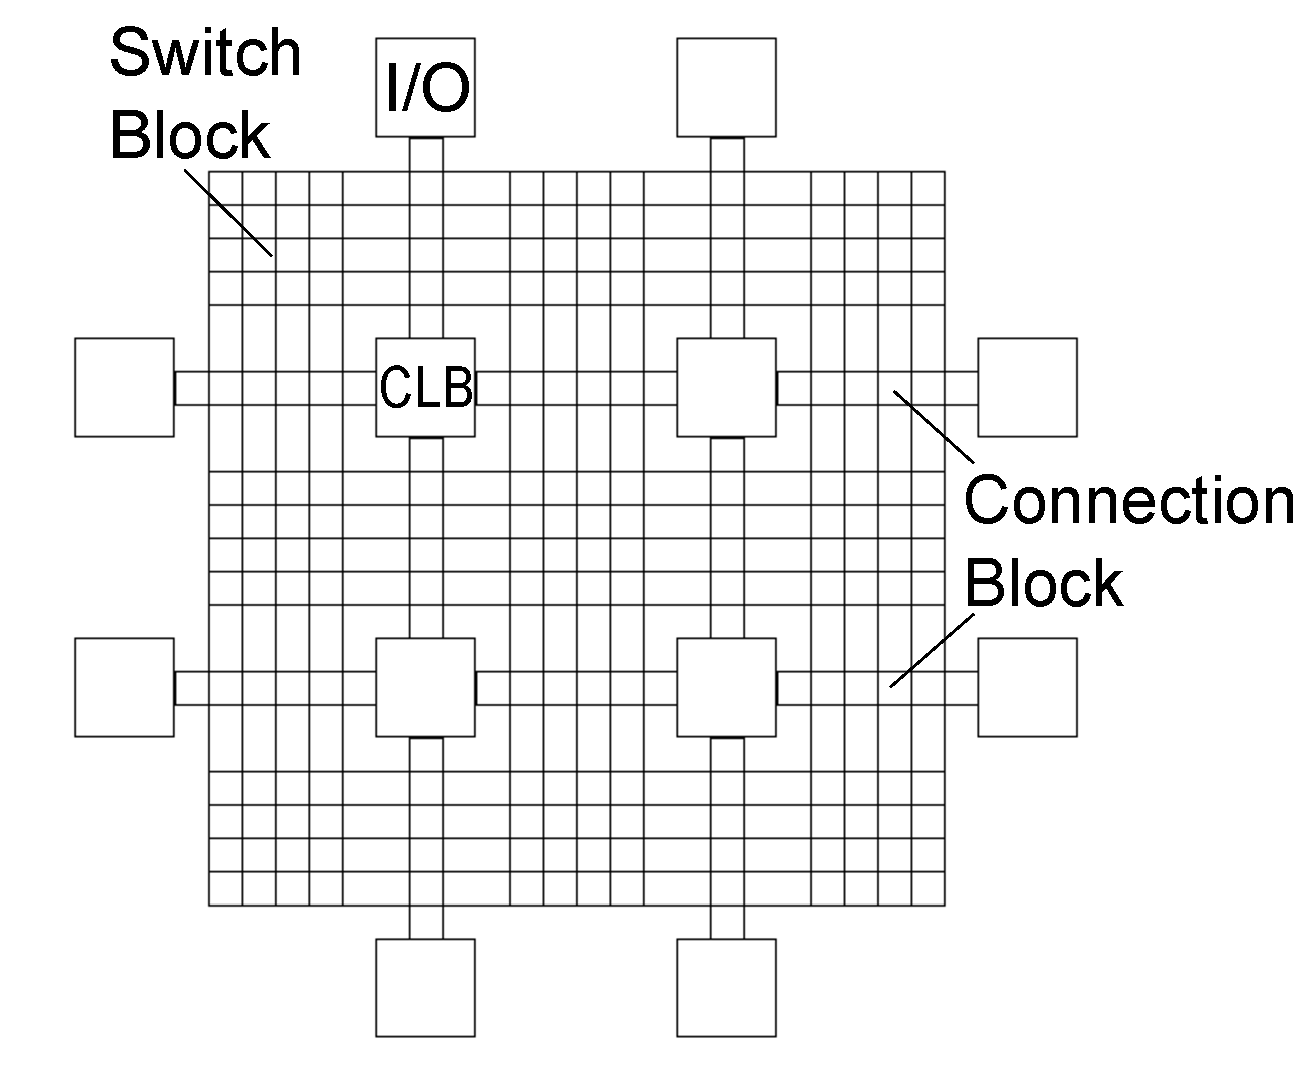
\includegraphics[width=0.6\textwidth]{images/ArchFull.pdf}
         \caption{Island Style FPGA} \label{FPGAArch} 
      \end{center}

   \end{figure}


   There are three main components to an \gls{FPGA}: \gls{IO} blocks, usually
   around the edge, allowing for input and output from the \gls{FPGA};
   \glspl{CLB} containing all the logic elements or \glspl{primitive}; and the
   routing between all the components.  Most \glspl{FPGA} also contain other
   structures embedded in the \gls{CLB} array to provide commonly used
   resources such as multipliers. While they can be implemented using registers
   and \glspl{LUT}, embedding them as discrete components allows for denser
   designs.  The routing between components consists of channels running
   horizontally and vertically with a number of wires and programmable switches
   connecting the wires to each other and to \glspl{CLB} allowing for
   configurable paths between arbitrary components. A typical switch or
   connection block has a configuration cell storing the state, and a
   connection can be made or unmade by writing a new value to the cell for that
   switch. The most common style of routing is known as island style (as the
   \glspl{CLB} are located as islands in a sea of routing) with the routing
   area making up some 80\%-90\% of the \gls{FPGA}'s area\cite{FPGAArch}.  Each
   \gls{CLB} is a cluster of smaller blocks, called \glspl{BLE}, with each
   \gls{BLE} containing the logic primitives, typically a programmable
   \gls{LUT} to implement combinational logic, a register for register operations
   and implementing sequential logic, and a \gls{mux} to switch between the
   two.
   
   The values for the \gls{LUT}, whether the \gls{mux} is selecting the
   register or \gls{LUT} output, and other component states are all stored in
   configuration memory like the routing switches and are typically implemented
   in \gls{SRAM}.
   
   Programming an \gls{FPGA} involves loading in a bitstream which describes
   all the component values (i.e. contents of the configuration memory for each
   cell) for a circuit, accomplished through writing the bitstream to a special
   configuration port on the \gls{FPGA}. A number of \glspl{FPGA} also allow
   for run time programming, or reconfiguration, of parts of a circuit through
   loading the bitstream for only the section of interest while the rest of the
   \gls{FPGA} keeps running.

   There are three main
   technologies used to implement the configuration memory in \glspl{FPGA}:

   \begin{itemize}

      \item \gls{SRAM}, which gives the highest density devices and includes
         the Virtex-5 family this thesis focuses on. These are volatile and
         must be reprogrammed every power up from an external configuration
         memory.
      \item (Anti)fuse, which are only one-time programmable.
      \item Flash, which is non-volatile (thus not does not require an external
         configuration memory) and reprogrammable. These have a lower
         density than \gls{SRAM} based \glspl{FPGA}\cite{FPGAArch}.

   \end{itemize}
   \subsubsection{Latch vs Flip-Flop}
   Typically, the register can implement either a latch or a flip-flop,
   as such future references to either latches or flip-flops both refer to a sequential logic element 
   implemented by a register.
   Generally the term latch is used for consistency with the language used by
   the \gls{BLIF} specification, and by \gls{VPR} and \gls{ABC}, although when discussing or referring to sources
   which use the term flip-flop the term flip-flop is also used.
   
   \subsubsection{Partial Reconfiguration} Partial
   reconfiguration involves loading configuration information for part of a
   circuit during operation. Much like the complete configuration described
   above, it involves writing a configuration bitstream to one of the
   available configuration ports, in this case also including the location
   of the region to reconfigure. The configuration memory of recent Virtex
   devices is subdivided into frames, and one can only reconfigure entire
   frames. A configuration frame is 41 (32-bit) words long on a Virtex-5
   device. The larger the area being reconfigured the more frames required,
   and consequently the larger the bitstream and hence the longer the time
   to reconfigure. The main configuration ports used are the external
   SelectMAP interface or the equivalent \gls{ICAP}, with a bandwidth of
   400MB/s in all Virtex devices \cite{XCell33,DiesselChange}



   \subsection{Space Based Applications}
   Space is quite different from a
   terrestrial environment, and \glspl{FPGA} have a number of advantages due to
   their lower \gls{NRE} costs and flexibility. As \glspl{FPGA} can be
   reconfigured during a mission, faulty or outdated designs can be replaced
   remotely; however, there is a significant downside: as systems go further
   into space and are no longer protected by the earth's atmosphere they become
   increasingly likely to suffer from radiation-induced errors where ionising
   radiation impinging on a component causes charge build up, potentially
   triggering incorrect operation\cite{SEEMechanism}. As outlined in Table
   \ref{SEURate}, for higher orbits the mean time to upset is on the order of
   only a second, and this rate increases as technology advances and chip
   density further increases.  
   \begin{table}

      \begin{center}


         \begin{tabular}
            {lll} \toprule Orbit & SEUs per device/day &Mean time
            to upset (s)\\
            \midrule LEO (560 km) & 4.09 & 2.11 $\times 10^4$\\

            Polar (833 km) & 1.49 $\times 10^4$ & 5.81\\
            GPS (20,200 km) & 5.46
            $\times 10^4$ & 1.58\\
            Geosynchronous (36,000 km) & 6.20 $\times
            10^4$ & 1.39\\
            \bottomrule 
         \end{tabular}
         \caption{SEU Rate
            Predictions for a Virtex-4 XC4VLX200 device at various
            orbits\cite{DiesselChange}} \label{SEURate} 


   \end{center}\end{table}
   Of the potential effects, which range from unnoticeable to
   device destruction, this thesis is concerned with mitigating \glspl{SEU},
   where an incorrect signal is triggered but the underlying circuitry is not
   damaged. We also concern ourselves primarily with errors affecting only
   single bits or components rather than \glspl{MBU} in which multiple
   components are affected at the same time.

   In an \gls{ASIC}, while \glspl{SEU} may be picked up and latched or
   otherwise continue affecting the circuit in future, the component itself
   continues operating normally.

   \glspl{FPGA} on the other hand are vulnerable to configuration errors as
   well. When the charged particle impacts configuration memory it can flip the
   state of that cell changing the implemented circuit. Unlike transient
   errors, these functional errors persist until corrected.

   Additionally for \gls{SRAM} devices, the off-chip configuration memory
   itself can be affected, so the next time the chip is reprogrammed (e.g.
   after power cycling), an incorrect circuit configuration will be loaded.

   (Anti)fuse devices, being non reprogrammable, are immune to configuration
   errors, though both \gls{SRAM} and flash-based \glspl{FPGA} are vulnerable
   and all three are susceptible to transient \glspl{SEU}\cite{HFPP}.


   \subsection{How We Deal With \gls{FPGA}
      Downsides} Clearly, in order for
   \glspl{FPGA} to be viable in space-based systems the effects of \glspl{SEU}
   must be mitigated. A number of technologies and techniques are available,
   each with their own advantages and disadvantages. A number of options exist
   which detect errors but are unable to determine the correct result,
   requiring a reload of the configuration memory while the circuit is non
   operational until the reconfiguration completes. For many applications this
   downtime is impractical, thus we will be looking at options which allow the
   circuit to continue operating correctly.  There are three main categories of
   \gls{SEU} hardening techniques for \glspl{FPGA}\cite{HardeningTechniques}:

   \begin{itemize}

      \item Charge Dissipation, which aims to keep the effect of the radiation
         below the level where it would have an effect. This includes
         techniques such as increasing the drive current. These methods
         typically require custom hardware (increasing costs) and usually
         increase power usage.
      \item Temporal Filtering, which aims to filter out transient \glspl{SEU},
         includes methods such as delay-and-vote\cite{HardeningTechniques}.
         These techniques often slow down operation and are ineffective
         against configuration errors.
      \item Spatial Redundancy, which uses multiple redundant circuits to
         detect errors and be able to continue operating. Spatial redundancy
         techniques include \gls{DICE}\cite{DICE} and \gls{TMR} and can be
         implemented either in hardware, or at the design level not
         requiring any custom hardware. These methods typically increase
         area and power usage.  
   \end{itemize}
   While hardened \glspl{FPGA}
   are available, they typically lag well behind mainstream commercial
   offerings\cite{VFPGATMR}, thus solutions which can be implemented on
   mainstream commercial \gls{FPGA} hardware are desirable. Additionally,
   there is very little point hardening an \gls{FPGA} and not its
   configuration buffers and memory which take up far more surface
   area\cite{FPGAArch} and are thus even more vulnerable.  For these reasons
   \gls{TMR}, requiring no custom hardware and providing \gls{SEU}
   protection against both transient and functional errors, is one of the
   more popular \gls{SEU} hardening techniques even though it comes at the
   cost of more than tripling area and greatly increasing power usage.
   Table \ref{HardeningComparison} details power usage, operating speed,
   hardness, and required area for flip flops which have been hardened using
   the techniques listing within the table. As can be seen, \gls{TMR} provides the greatest hardness
   (measured as the greatest average time between errors) at the cost of the highest overhead in power and area usage.
   \begin{table}
      \begin{center}


      \begin{tabularx}
         {\textwidth}{X|RRRRR} \toprule & Power ($\mu$W) & Speed
         (ns) & Hardness (errors per bit-day) & Node Failures Required for Device Failure & Area ($\mbox{$\mu$m}^2$)\\
         \midrule Standard
         & Rise – 0.7\newline Fall – 0.2 & Rise – 0.21\newline Fall – 0.27&
         $10^{-8}$ & 1 & 360\\
         \midrule Increased Drive Current
         & Rise – 1.0\newline Fall – 0.2 & Rise – 0.16\newline Fall – 0.15&
         $2\times10^{-9}$ & 1 & 460\\
         \midrule \gls{TMR} & Rise
         – 1.72\newline Fall – 1.27 & Rise – 0.2\newline Fall – 0.27 &
         $10^{-11}$ & 2& 1200\\
         \midrule \gls{DICE} & Rise -
         1.4\newline Fall - 1.1 & Rise - 0.96\newline Fall - 0.97&
         $1.6\times10^{-10}$& 2 & 520 \\
         \bottomrule

      \end{tabularx}
      \caption{Comparison of hardening
         techniques\cite{HardeningTechniques}} \label{HardeningComparison}

   \end{center}\end{table}
   Additionally, for \gls{SRAM}
   based \glspl{FPGA} the off-chip configuration memory must also be
   protected as \gls{SRAM} is volatile and loads the state from this memory
   at start up. This can be accomplished by incorporating error detection
   and correction techniques in the RAM, something already in place on a
   number of mainstream \glspl{FPGA} such as the Virtex-4 and
   -5\cite{DuttonSEU}.

   One additional type of hardening is physical shielding i.e. surrounding the
   \gls{FPGA} with a material to block incoming radiation. Unlike the above
   approaches this requires no modification to the \gls{FPGA} hardware or
   implemented circuit. Unfortunately, it increases cost, weight and size, and
   may not always be practical. \fxwarning{Expand?}

   \glsunset{TMR} 
   \section{\gls{TMR}
   }\label{secTMR} Triple Modular Redundancy is a
   commonly used method for creating fault tolerant systems in which a given
   circuit is implemented three times with independent components, with the
   outputs feeding into a voter circuit to determine the majority value. As an
   \gls{SEU} affects only a single component or bit of data it
   will affect the output value of at most one version, so the majority vote is
   still correct. For transient errors that are not in a feedback loop correcting
   the output is enough to fix the error; however, \glspl{SEU} in feedback paths
   or in the configuration memory will persist, and this necessitates some method
   for eliminating them. One possible approach is resetting the system but while
   this occurs the system is unavailable, so a reset may not be a feasible
   solution. Instead, partial reconfiguration could be used to reconfigure only
   the faulty circuit while the redundant circuits continue operating and
   providing output. After reconfiguration the circuit must then be resynchronised
   to the same state as the other two. We use the approach presented by
   \cite{DiesselChange} which involves running the circuit until the state
   converges, which is guaranteed (for acyclic circuits) to occur within a
   timeframe given by the number of register stages (also referred to as critical path length)
    and the clock period. In
   order for this approach to always resynchronise correctly the circuit must have
   no feedback loops which could carry incorrect data. To solve this we simply
   ensure that all feedback loops are \textit{cut}, that is, the value is voted on
   before being passed back into the circuit. This has the additional benefit of
   correcting transient errors which would otherwise be caught in a feedback cycle
   by ensuring the cycle data is correct.

   This approach requires three times as many circuit elements (as the circuits
   are triplicated) plus whatever is required for voters. By minimising the
   number of voters, we can thus reduce the overhead of our approach.

   \subsection{Error Recovery Time for \gls{TMR}}

   Once an error occurs it takes up to $T_{path}$ to reach the voter and be
   detected, where $T_{path}$ is given by the clock period and number of
   register stages. This is called the \textit{error detection time}. Detection
   of an error can then be used to trigger reconfiguration.

   Sending a request to the reconfiguration controller goes through a token
   ring network connecting together the other voters and the reconfiguration
   controller. In the worst case it takes one full cycle of the network to
   receive the token, one full cycle to reach the reconfiguration controller,
   and three cycles to transmit the request, giving $5\times Cycles Per Hop$.
   Benchmarks of a sample voter indicate 50 clock cycles per hop is a good
   estimate.

   Reconfiguration time is dependent upon the circuit size.
   For our target device based on Virtex-5 we round the circuit's area usage up
   to an allocatable area of 20 \glspl{CLB} (representing one column of \glspl{CLB} 
   in a reconfiguration row). Each \gls{CLB} consists of 8 \glspl{BLE} (each
   \gls{BLE} having one \gls{LUT} and one latch) giving us a target 
   reconfiguration area that consists of 160 \glspl{BLE} and requiring 36
   frames of 41 32-bit words each. The bitstream size for this area is 1476
   words which takes 14.8$\mu{}s$ to reconfigure at 100MHz
   \cite{XilinxConfigurationUG}.  Once the error has been detected and the
   circuit reconfigured it must then be resynchronised with the other
   partitions, which takes up to $T_{path}$ using the previously described
   technique.

   The error recovery time consists of the time to detect the error, send a
   request to the configuration controller, and then reconfigure and
   resynchronise the circuit, thus is a function of the circuit area, clock
   period, and number of register stages. Therefore it is required that the
   number of register stages and area are small enough,
   that our error recovery time is within a user specified limit.

   \begin{align}
      \mbox{Error Recovery Time} &=\mbox{Error Detection Time} +\mbox{Communication Time} \notag\\
      &+\mbox{Reconfiguration Time} + \mbox{Resynchronisation Time}\notag\\
      \mbox{Error Detection Time} &\le T_{path} = \mbox{Clock
         Period}\times\mbox{Register Stages}\notag\\
      \mbox{Communication Time}
      &\le 5\times \mbox{Cycles per hop}\times\mbox{Number of Hops}\times \mbox{Clock Period}\notag\\
      &= 50\times 5\times (\mbox{Number of
         Partitions}+1)\times \mbox{Clock Period}\notag\\
      \mbox{Reconfiguration
         Time} &= \frac{\mbox{Bitstream
            Size}}{\mbox{Reconfiguration Speed}}\notag\\
      &=\left\lceil \frac{\mbox{Number of
            \glspl{BLE}}}{160}\right\rceil\times 1.48\times10^{-5}\notag\\
      \mbox{Resynchronisation Time} &\le T_{path} = \mbox{Clock
         Period}\times\mbox{Register Stages}\notag\\
   \end{align}
   
   While most of the values used are directly calculable, the number of partitions and the circuit clock period are
   not known until after partitioning and after routing respectively and must therefore be estimated.
   The estimations used in our implementation are described in Section \ref{DesignEstimates}.


   Additionally, as each voter circuit adds some constant overhead in terms of
   area, power usage and clock period slowdown it is desirable to have each
   partition as large as possible. This thesis is concerned with implementing
   and assessing this \gls{TMR} design; a discussion of other \gls{TMR} methods
   and our reasons for not using them is included below.

   This method only works when at most one \gls{SEU} occurs within the error
   detection and recovery time; should \glspl{SEU} occur in two of the three
   partitions then it is impossible for the voter to determine the correct
   value necessitating a complete reload of the configuration memory
   (\gls{scrubbing}). Therefore, we require the error detection and recovery
   time to be sufficiently small that the likelihood of multiple events
   occurring within that time period is minimised.

   Additionally, as mentioned earlier, it is also desirable to minimise the
   number of voters to reduce the overhead of this approach. To that end,
   having larger (and hence fewer) partitions is preferable to smaller
   partitions provided we still stay within our target recovery time.

   \glsunset{TMR} 
   \subsection{\gls{TMR}
      Implementations} This thesis builds on the
   work of\cite{DiesselChange} which describes a partitioning algorithm that
   traverses a circuit represented as a \gls{DFG} in a breadth-first manner,
   creating partitions that stay within our constraints.  Our goal is to create an
   algorithm which stays within a user-specified error recovery time, doesn't
   require existing code to be rewritten, allows for both custom voting and
   reconfiguration logic to be added, can use industry standard \glspl{FPGA}
   rather than custom hardware, and effectively protects the entire system from
   \glspl{SEU} with as close to no downtime as achievable.  Additionally, it is
   desirable to limit the overhead of implementing \gls{TMR} through minimising
   the number of voters required.  There are a number of existing \gls{TMR}
   solutions, but none quite meet our requirements.  Our first requirement is
   that standard \gls{FPGA} hardware can be used, with our implementation
   specifically targeting Virtex-5 chips. Options with custom hardware such as
   \cite{VFPGATMR} (with three \glspl{FPGA} and an \gls{ASIC} voter in a single
   package), are often prohibitively expensive, and prevent us from using our
   existing boards.  Many \glspl{FPGA} marketed specifically at space-based
   applications are, in addition to featuring specialised hardware, only
   latchup immune or only include inbuilt \gls{TMR} on registers,
   leaving them still vulnerable to \glspl{SEU} \cite{FPGAReview}.  Non-hardware
   solutions are typically implemented pre-synthesis, such as \cite{ftmr} (which
   introduces a \gls{VHDL} library featuring triplicated components), and require
   existing code to be rewritten, or during synthesis such as \cite{synplify} and
   \cite{tmrtool}, neither of which supports specifying an error recovery limit, nor
   for adding reconfiguration logic.  Other options look at using partial
   \gls{TMR} (such as \cite{partialTMR}) which, while it does reduce the overhead
   of \gls{TMR}, means the entire circuit is no longer protected, or have
   excessive downtimes to recover from errors such as \cite{VTMR}, which uses idle
   cycles in a data path to calculate redundant results.  One approach similar to
   ours is presented by \cite{PostSynth} who also partition a post-synthesis
   netlist (represented by a \gls{DFG}), but their focus is on evaluating
   techniques for cutting feedback loops, while we focus on partitioning circuits
   into smaller sub circuits. Cutting feedback loops is however a part of this
   thesis, and their work could be incorporated in, although for our current
   implementation a simple depth-first traversal described later in Chapter \ref{algorithm} was chosen.


   \subsection{Our Algorithm}
   \label{Algorithm} 
   \begin{figure}

      \begin{center}

         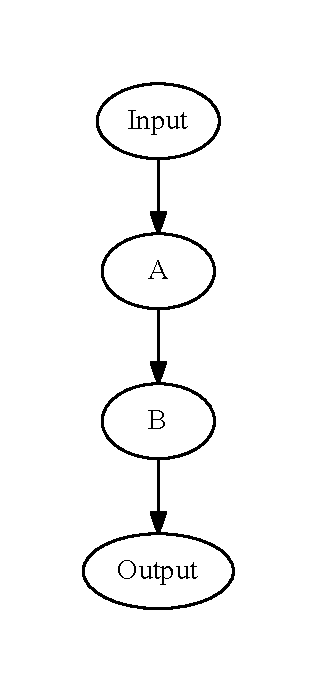
\includegraphics[height=0.3\textheight]{images/TMR-graph.pdf}
         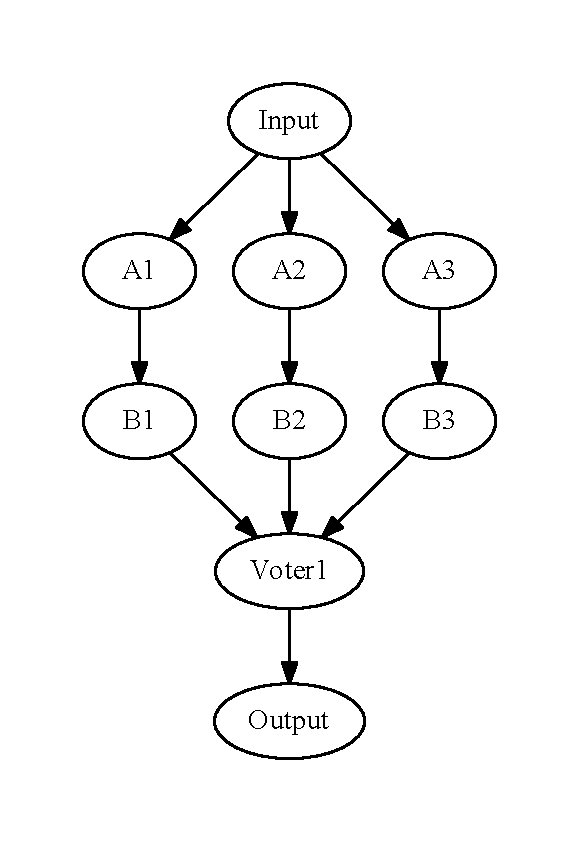
\includegraphics[height=0.3\textheight]{images/TMR-post.pdf}
         \caption{\gls{DFG} before and after partitioning} \label{TMRFigure}

      \end{center}

   \end{figure}
   Given a netlist description of a circuit, it is
   possible to represent the circuit as a \gls{DFG}\cite{FPGAArch}. Our goal is
   to split a \gls{DFG} into a number of smaller subgraphs, triplicate the
   components of each subgraph, and insert voting and recovery logic, with each
   subgraph having independent components and an error recovery time within our
   threshold. We can then proceed to implement our graph, made up of our new
   subgraphs, as normal.  To do so we traverse the \gls{DFG} in a depth-first
   manner, keeping track of the number of register stages and area,
   extending our partition area as we do so, until our recovery time
   constraint would be violated.  As we extend our partition area we must
   detect any cycles within our current partition and cut them, joining them back up after the output has
   been voted on. We thereby ensure that each partition is acyclic and
   guarantee that the circuit will resynchronise and not get incorrect data
   trapped in a feedback loop.  At that point we cleave off our partition and
   write it to a file, open a new empty partition, and repeat for all circuit
   elements.  Once this is done, we have a set of subcircuits. We now
   triplicate each partition and insert our additional voting logic, then join
   each subcircuit back together.

   \glsunset{CAD} 
   \section{\gls{CAD}
      Flow} \glspl{FPGA} are typically programmed
   in a hardware description language such as \gls{VHDL} or Verilog, and then a
   number of programs (collectively making up the \gls{CAD} flow or development
   toolchain) turn the source into a bitstream to program a target \gls{FPGA}.
   The design flow process can be split into a number of
   subprocesses as illustrated in Figure
   \ref{CADFlow}\cite{VPRBook,VPRManual,FPGAArch}.  
   \begin{enumerate}

      \item The synthesiser turns a hardware description language such as VHDL
         or Verilog into a netlist of basic gates and flip-flops.
      \item The optimiser removes redundant logic, and attempts to simplify
         logic.
      \item The mapper maps logic elements to \glspl{primitive}, the basic
         logic elements contained on the \gls{FPGA}.
      \item The packer combines logic elements into \glspl{CLB}.
      \item The placer locates each \gls{CLB} within the \gls{FPGA}
         architecture, deciding which physical block implements which logic
         block.
      \item The router makes the required connections between each element by
         deciding which switches are on or off. This includes the
         connections within each \gls{CLB} (local routing) and between
         \glspl{CLB} (global routing).  
   \end{enumerate}
   For our partitioner
   we will insert an additional step into the design flow between mapping
   and packing, which operates directly on a netlist. The additional steps
   are detailed in Chapter \ref{algorithm}.


   \begin{figure}

      \begin{center}
         \includegraphics*[viewport=40 280 550 750]{images/VPRCAD.pdf}
         \caption{Cad Design Flow.\cite{VPRManual}} \label{CADFlow}

      \end{center}

   \end{figure}
   \glsunset{VPR} 
   \subsection{How \gls{VPR} Works}
   \label{VPRSection} For this thesis we will be assessing the results
   of our algorithm implementation after processing by \gls{VPR}, an open-source packer, placer and router. \gls{VPR} was chosen as the algorithms
   used are public and well documented, it is open source allowing
   modifications to be made if necessary, and it is well documented and popular
   in research, making it much easier for us to determine what's happening and
   why, rather than relying on proprietary black box processes from commercial
   vendors. Additionally, \gls{BLIF} (the format used by \gls{VPR}) benchmarks
   are readily available.  A brief understanding of the algorithms used in
   \gls{VPR} and the effects of different settings is useful, though not
   critical, for understanding the results. \cite{VPRManual} has a more
   detailed list of all the options \gls{VPR} takes. Unless otherwise
   specified, all values are at their defaults.  \subsubsection{Packer}
   \gls{VPR} uses the AAPack algorithm described by \cite{AAPackThesis}. This
   is a greedy algorithm which operates on blocks sequentially, starting with
   an \gls{FPGA} area of 1 block by 1 block. For each block it greedily adds
   \textit{primitives} (latches or \glspl{LUT}) based on a configurable cost
   function until no more primitives can be added. It then repeats for the next
   block, and the next after that, until every primitive has been packed. As it
   runs out of blocks in the current \gls{FPGA} area it expands the \gls{FPGA}
   area used until it reaches the physical limit specified in the architecture
   file (or grows indefinitely if no limit is specified). This means that even
   if the device is of area 40 by 40, if the packer can fit everything in a 30
   by 30 area it will do so, and \gls{VPR} will treat the \gls{FPGA} as being
   only 30 by 30.  The cost function can be configured through options passed
   to \gls{VPR}, to\cite{VPRManual}: 
   \begin{itemize}

      \item prioritise optimisation of timing or area (default is prefer
         timing)
      \item prioritise absorbing nets with fewer connections over those with
         more (default is yes)
      \item when prioritising absorbing nets with fewer connections, focus more
         on signal sharing or absorbing smaller nets (default is greatly
         prefer absorbing smaller nets)
      \item determine the next complex block to pack based on timing or number
         of inputs (default is timing).  
   \end{itemize}
   The main thing to
   note, as relates to our results, is that as much as possible AAPack will
   never leave blocks partially packed while there is still a primitive
   which will fit. Even when optimising timing exclusively, it will still
   attempt to maximally pack each cluster even if it negatively impacts circuit performance.

   \subsubsection{Placer} \gls{VPR}'s placer uses a simulated annealing
   algorithm where the options allow us to specify annealing schedule
   parameters and cost function. The default options were chosen via
   experimentation and are likely superior to custom options we may choose to
   use, and affect the average quality of the result rather than materially
   affecting the behaviour \cite{VPRManual, VPRBook}. For these reasons we will
   be leaving them at their default. Section \ref{stochastic} discusses the
   variation in results due to the stochastic nature of the placement
   algorithm.
   \subsubsection{Router} \gls{VPR}'s router supports three
   different algorithms: breadth\_first, which
   focuses solely on routing a design; timing\_driven, the default, which tends
   to use slightly more tracks (~5\%) than breadth\_first while providing much
   faster routes (2$\times$--10$\times$) with less CPU time; and
   directed\_search, which like breadth\_first is routability driven however
   uses A* to improve runtime. We will be using the default timing\_driven
   algorithm. There are a number of other options setting
   algorithm parameters, all of which we will leave at their defaults.
   Additionally, we can set the width of the architecture's routing channels through the
   route\_chan\_width parameter.
   If omitted \gls{VPR} will perform a binary search on channel capacity to
   determine the minimum channel width.


   \chapter{Project Outline}

   \section{Project Objectives}
   \label{secObjectives}
   The objective of this thesis is to create an implementation of the algorithm
   outlined by \cite{DiesselChange} and assess the overheads of this method.  As
   such, we need to create a \textit{correct} implementation, that is, one which
   :
   \begin{enumerate}

      \item Correctly implements TMR.
      \item Preserves the original inputs and outputs. Signals should retain
         the same names, and for a set of inputs, the circuit should have
         the same output as the original circuit.
      \item Is accurate in partitioning, such that subpartitions are all
         within the target recovery time.  
   \end{enumerate}
   and then
   evaluate the overhead of this algorithm in terms of algorithm running
   time, and how it affects the performance of the final circuit.

   \section{Design of Partitioning Algorithm} \label{DesignEstimates}
    Chapter \ref{algorithm} describes the partitioning algorithm fully; in brief our design is to:
    \begin{enumerate}
    	\item Split a larger input circuit into smaller partitions
    	\item Triplicate each partition
    	\item Join them back together.
\end{enumerate}
    While splitting our design into smaller partitions we need to cut any cycles internal to a partition such that they pass through
    the voter circuit and then the corrected output is fed back into the partition.
    
    The size of each partition is set such that each partition has an error recovery time less than a user specified target.
    The error recovery time is calculated as per Section \ref{secTMR} with estimates for the number of partitions and final circuit clock period as follows:
    An initial guess for the final number of partitions is set at 1, and the partitioner is run to completion.
    The guess is then updated to the actual number of generated partitions and the partitioner is rerun. This repeats until the guess is the same or greater than the actual generated number of partitions, or partitions within the target recovery time were unable to be created.
    In practice, it generally only takes two or three runs to converge to the actual number of partitions for the twenty largest \gls{MCNC} benchmarks although some tested corner cases took up to ten repetitions on increasing estimates before the partitioner determined that the target recovery time was unable to be met.
    As all target benchmark circuits completed partitioning relatively quickly and it is impossible for the partitioner to be stuck in an infinite loop of revising its estimate optimising this estimation was not considered necessary.
    
    In addition to an estimate for the number of partitions, to calculate the recovery time the partitioner requires an estimate for the final clock period. This is derived as $1.8\times$ the original circuit's clock period, as reported by \gls{VPR} upon processing the original circuit. 1.8 was experimentally chosen, as the all the circuits were under an average $1.8\times$ slowdown, and the average case was well under.
    
   \glsunset{CPU}
   \section{Assessment of
      Partitioning Algorithm} Assessment is based on the fulfillment of
   the criteria outlined earlier in this chapter, in Section
   \ref{secObjectives} as they relate to a set of benchmark circuits, the
   twenty largest MCNC circuits from LGSYNTH'93.  Generated circuits were
   verified against and compared with the original circuits to confirm
   that the algorithm operated correctly, as described further in Section
   \ref{secTesting}.  The \gls{CPU} time of
   the algorithm as it runs against the benchmarks was recorded and
   compared with the running time of \gls{VPR} as detailed in Section
   \ref{timing}. And lastly, the
   performance of the generated circuits was compared to the original
   untriplicated circuits in Chapter \ref{results}.



   \chapter{Algorithm}\label{algorithm}
   For our partitioner, we operate on a netlist in
   \gls{BLIF} format (described in Section \ref{secBlif}) after optimisation
   and technology mapping, but before packing. Our goal is to take an input
   netlist and transform it into a netlist in the same format, with the same
   set of outputs for each set of inputs, but with redundant components.

   \begin{figure}

      \begin{center}

         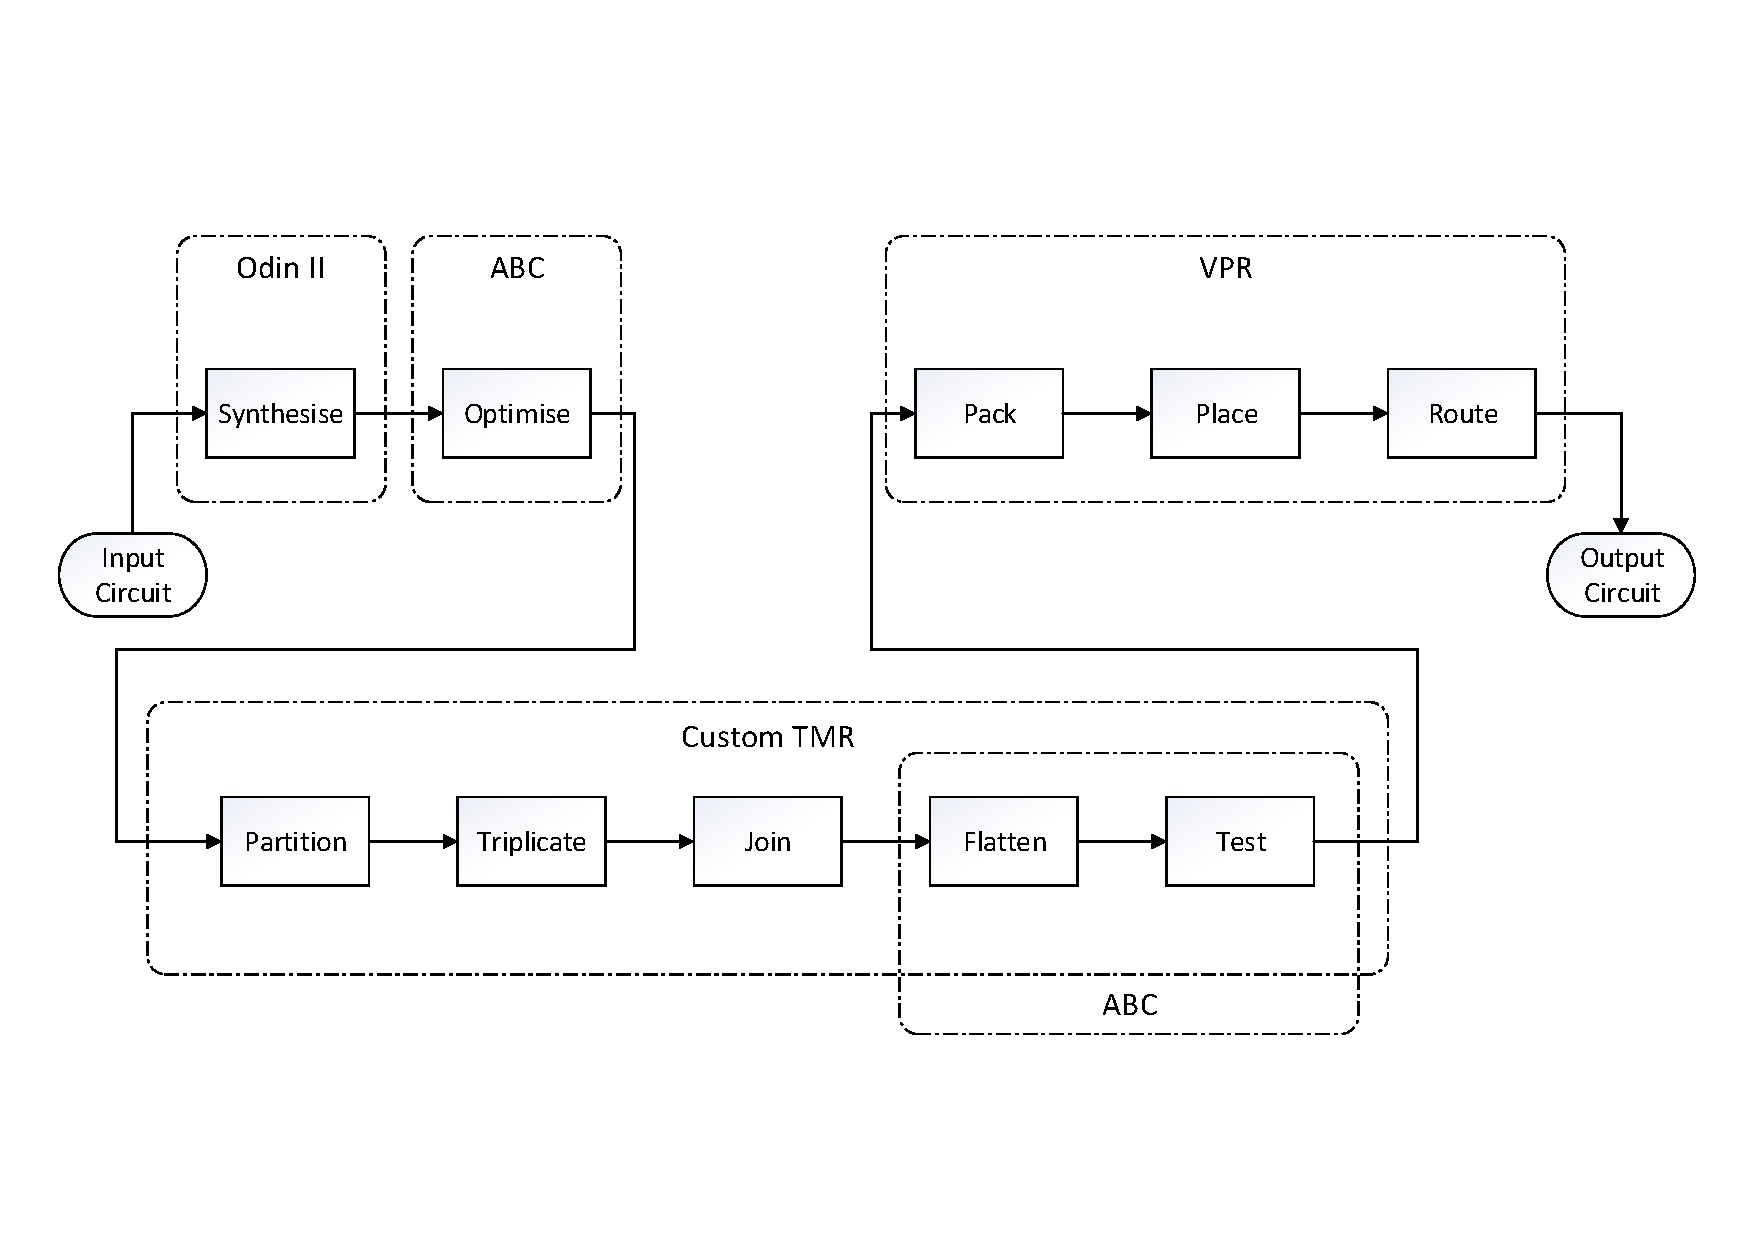
\includegraphics[width=\linewidth]{images/CadFlowWPartitioner.pdf}
         \caption{Custom Tool Flow} \label{algToolflow} 
      \end{center}


   \end{figure}
   Figure \ref{algToolflow} illustrates a typical \gls{CAD} toolchain with our
   custom partitioner added and the substeps expanded (c.f. Figure
   \ref{CADFlow} for an example without). The steps below are explained in more
   detail in Section \ref{secAlgorithm}.
   \begin{itemize}

      \item Partition - Take an input circuit and split it into multiple
         smaller circuits, one per file.
      \item Triplicate - Take an input circuit and transform it into a TMR'd
         version.
      \item Join - Take a set of input files, one circuit per file, and join
         them into one larger circuit by joining corresponding signals.
      \item Flatten - Use \GLS{ABC} to transform a heirarchical circuit into a
         format supported by VPR.
      \item Test - Use the verification capability of \gls{ABC} to verify that
         the generated circuit is equivalent to the original.  
   \end{itemize}

\FloatBarrier
   \section{Data Structures}
   \label{secDatastructures} 
   \subsection{Basic Types}

   Table \ref{basicTypes} lists the basic types, out of which others are built.
   There is generally, but not always, a direct
   relationship to a C++ primitive.  
   \begin{table}
      \begin{center}


      \begin{tabularx}
         {\linewidth}{XXX} \toprule Name & Closest C++ Equivalent
         & Description\\
         \midrule \textbf{Integer} &  int & Whole number \\
         \textbf{Boolean} &
         bool & True or False \\
         \textbf{Float} & float & Floating point number \\
         \textbf{Queue}
         & std::list & FIFO queue \\
         \textbf{List(type)} &
         std::list$\langle$type$\rangle$ & \\
         \textbf{String} & std::string & String
         object that provides operations to manipulate itself \\
         \textbf{File} &
         std::iostream & Abstract type to represent simple I/O operations \\

         \textbf{Map(KeyType $\to$ ValueType, DEFAULT:  DefaultValue)} &
         std::unordered\_map$\langle$KeyType, ValueType$\rangle$ &  A map to
         translate values of type KeyType to values of type ValueType. If the
         key isn't present, returns DefaultValue \\
         \bottomrule 
      \end{tabularx}

      \caption{Basic Data Types} \label{basicTypes}
   \end{center}\end{table}
   Table \ref{complexTypes} contains an overview of the custom complex
   types, which are further explained below.
   \begin{table}
      \begin{center}

      \begin{tabularx}
         {\linewidth}{lX} \toprule Name &
         Description\\
         \midrule
         \textbf{Blif} & Parent object, contains all information
         about a \gls{BLIF} file and provides useful operations \\
         \textbf{Model} &
         Represents a circuit within a \gls{BLIF} file, and provides methods to
         manipulate said circuit \\
         \textbf{BlifNode} & A circuit element, or node in
         the \gls{DFG} representing the circuit \\
         \textbf{Signa}l & A signal within a
         specific circuit, or Model, representing a set of edges with common
         source \\
         \bottomrule 
      \end{tabularx}
      \caption{Complex Data Types}\label{complexTypes}

   \end{center}\end{table}
\fxnote{Bold types in text?}



   \subsection{Blif}
   Contains helper functions to read in a \gls{BLIF} and
   represent it as a \gls{DFG}.  The circuit itself is represented as a Model
   within Blif.  
   \begin{table}
      \begin{center}

      \begin{tabularx}
         {\linewidth}{llX} \toprule Field
         Name & Type & Description\\
         \midrule masterOutputs &
         \textbf{List(String)} & List of outputs for the original file \\

         masterInputs & \textbf{List(String)} & List of inputs for the original
         file \\
         main & \textbf{Model} & The main circuit in the \gls{BLIF}
         file\\
         \bottomrule 
      \end{tabularx}
      \caption{Fields in Blif object}

   \end{center}\end{table}



   \subsection{Model}
   Represents the circuit as a \gls{DFG}, with a list of
   BlifNodes and the Signals both between nodes, and the primary inputs/outputs
   of the circuit.  Also contains a mapping from Signal name to Signal.

   \begin{table}
      \begin{center}

      \begin{tabularx}
         {\linewidth}{lXX} \toprule Field Name & Type &
         Description\\
         \midrule name & \textbf{String} & Name of the circuit
         \\
         signals & \textbf{Map(String $\to$ Signal, DEFAULT: NULL)} & Map
         from signal name to Signal object \\
         outputs & \textbf{List(Signal)} &
         List of output Signal objects \\
         inputs & \textbf{List(Signal)} & List
         of input Signal objects \\
         nodes & \textbf{List(BlifNode)} & List of
         all nodes in a circuit \\
         numLatches & \textbf{Integer} & Number of
         latches within a circuit \\
         numLUTs & \textbf{Integer} & Number of
         LUTs within a circuit \\
         \bottomrule 
      \end{tabularx}
      \caption{Fields in
         Model object} 
   \end{center}\end{table}



   \subsection{BlifNode}
   Contains the names of the input and output Signals, as
   well as the properties of the node (type, etc).  Does not contain direct
   references to Signals, merely their names.  
   \begin{table}
      \begin{center}


      \begin{tabularx}
         {\linewidth}{llX} \toprule Field Name & Type &
         Description\\
         \midrule output & \textbf{String} & Name of output
         signal \\
         clock & \textbf{String} & Name of clock signal \\
         inputs &
         \textbf{List(String)} & List of input signal names \\
         cost & \textbf{Integer} & How many clock cycles this node contributes to the
         critical path. 0 for \glspl{LUT} and 1 for latches. \\
         type & \textbf{String} & Type of node, ``latch'' or ``names'' (\gls{LUT}) \\

         contents & \textbf{String} & Parameters describing node which are not
         used by partitioner but required to recreate \gls{BLIF} file e.g.
         initial latch state\\
         \bottomrule 
      \end{tabularx}
      \caption{Fields in
         BlifNode object} 
   \end{center}\end{table}



   \subsection{Signal}
   Contains references to the signal source, and a list of
   its sinks. Also stores the signal name.  
   \begin{table}
   \begin{center}


      \begin{tabularx}
         {\linewidth}{llX} \toprule Field Name & Type &
         Description\\
         \midrule name & \textbf{String} & Name of the signal \\

         source & \textbf{BlifNode} & Pointer to source node which drives this
         signal \\
         sinks & \textbf{List(BlifNode)} & List of pointers to this
         node's sinks.\\
         \bottomrule 
      \end{tabularx}
      \caption{Fields in Signal
         object} 
   \end{center}\end{table}



   \subsection{\gls{DFG}
      Traversal} BlifNodes represent nodes in the \gls{DFG}
   while Signals represent a collection of edges with common source. Traversing
   the network is thus achieved through traversing from node$\rightarrow$
   signal$\rightarrow$ node. However, \mbox{BlifNodes} do not store a pointer to the
   Signal, just the name of the Signal. The actual Signal object, being
   specific to a partition while BlifNodes are not (nodes can be added to and
   removed from Models with no issue, and can even exist in multiple at once
   e.g. original circuit and subpartition). This means that signals must be
   looked up in the partition by name. To this end, Model contains a field \textit{signals}
    which is a map from signal name to Signal.

   Thus, an example which recursively traverses from a node to its children
   would be: 
\renewcommand\algorithmiccomment[1]{%
  \hfill$\triangleright$\ \parbox[t]{.40\linewidth}{#1}%
}
   \begin{algorithm}
      \caption{Example Traversal}\label{algExTrav}

      \begin{algorithmic}[1]
      \Procedure{ExampleTraversal}{$startNode$,
            $partition$} 
            \State $\triangleright$ Get the name of our output signal
         \State $outputName \gets startNode.output$
         \State
            \State $\triangleright$ From a Signal name, get the
            Signal object
         \State $outputSignal \gets         partition.signals[outputName]$
         \State
            \State $\triangleright$ Retrieve the sinks of a signal, which are also the immediate
            childen of our start node
            \ForAll{$childNode \in outputSignal.sinks$}
         \State Print(``Reached childNode from startNode'')
         \State
            \State $\triangleright$ Recursively visit the child
         \State ExampleTraversal$(childNode, partition)$
          \EndFor
           \EndProcedure

      \end{algorithmic}

   \end{algorithm}


\renewcommand\algorithmiccomment[1]{%
  \hfill$\triangleright$\ \parbox[t]{.25\linewidth}{#1}%
}
   Given a Model which represents the circuit as a DFG and contains a list of nodes, map of signal
   name $\to$ Signal, and lists of primary inputs and outputs for the circuit,
   each node contains the names of its input and output signals, allowing the
   Signal to be looked up, and the Signal contains pointers to its source and
   sink nodes.  This allows the DFG to be traversed by going from node, to
   signal, to node, etc.  A BlifNode represents the information in a circuit
   element declaration within a \gls{BLIF} file, which includes only the name
   of its input and output signals. The actual Signal itself is a separate
   circuit specific construct designed to allow for ease of traversal of the
   circuit as a \gls{DFG}.  As such, we don't directly point to signals from a
   BlifNode, as the Signal depends on the circuit context.  \fixme{TODO: Image
      showing DFG traversal, and example of blif file and class contents}

   \newpage 
   \section{Algorithm}
   \label{secAlgorithm} 
   \subsection{Main}

   Partition, Triplicate, Join and Flatten are all implemented in separate
   programs. Main is responsible for taking an input file and running it
   through our toolchain to produce a TMR'd output file.



   \begin{algorithm}

      \begin{center}

         \begin{tabular}
            {lll} \toprule Variable &
            Type & Description\\
            \midrule $input$ & \textbf{File} &  Input blif
            file\\
            $targetRecoveryTime$ & \textbf{Float} &  Per partition
            recovery time (in seconds) \\
            $files$ & \textbf{List(File)} &
            circuit partitions, one per file \\
            $file$ & \textbf{File} &  \\

            $header$ & \textbf{String} &  string containing the first three
            lines of the input file \\
            $output$ & \textbf{File} &  output
            file\\
            \bottomrule 
         \end{tabular}

      \end{center}
      \caption{Main
         Algorithm}\label{main} 
      \begin{algorithmic}[1]
         \Procedure{Main}{$input$, $targetRecoveryTime$} 
         \State $baseClockPeriod \gets $VPR$(input)$
         \State $files \gets
         \mbox{Partition}(input, targetRecoveryTime, baseClockPeriod\times1.8)$ \ForAll {$file \in
            files$} 
         \State $file \gets \mbox{Triplicate}(file)$ \EndFor 
         \State
         $header \gets input.lines[0\to 3]$ 
         \State $file \gets
         \mbox{Join}(files, header)$ 
         \State $output \gets
         \mbox{Flatten}(output)$ \EndProcedure 
      \end{algorithmic}


   \end{algorithm}
   We're given a blif file as input.
   First, in line 2 we run the original circuit through \gls{VPR} to determine the clock period of the base circuit.
   In line 3 we partition the input circuit into a number of sub circuits, each in a separate file, as
   further expanded in Algorithm \ref{partition}, passing it our target recovery time, and an estimate of the final circuit's clock period.
   Then in lines 4-5 for each
   partition file we read it in as a black box, triplicate it, insert voting
   logic, and write it back out.  Next in line 7 we extract the original
   header, which provides the name, inputs and outputs of the original circuit.
   We then, in line 8, join all the partitions together with the original name,
   inputs and outputs (in the same order), as the original circuit, and finally
   line 8 flattens the circuit, i.e. transforms the generated hierarchical
   netlist into a flat netlist with only one main model, or circuit, and no
   submodels.

   \newpage 
   \subsection{Partition}
   \label{algPartition} Given an input file,
   Partition reads it in, and splits it into a number of smaller subcircuits,
   each of which has a maximum recovery time of our target recovery time or
   less. Each subcircuit is then output to its own separate file, each of which
   is a valid \gls{BLIF} circuit on its own.  
   \begin{table}

      \begin{center}


         \begin{tabularx}
            {\linewidth}{llX} \toprule Variable & Type &
            Description\\
            \midrule $file$ &\textbf{File  } &  input file\\
            $targetRecoveryTime$ &\textbf{Float } &  maximum per partition
            recovery time (in seconds)\\
            $estimatedClockPeriod$ &\textbf{Float} & An estimate for the final clock period of the partitioned circuit\\
            $blif$ &\textbf{Blif } &  In-memory
            representation of input blif file\\
            $circuit$ &\textbf{Model }
            &  Main circuit from input file, represented as DFG\\
            targetPartitions & \textbf{Integer} & An estimate for the number of partitions \\
            $partition$
            &\textbf{Model } &  Circuit, which we are adding nodes to, to
            make our partition\\
            $queue$ &\textbf{Queue } &  FIFO queue of
            nodes to visit\\
            $visited$ &\textbf{Map(BlifNode$\to$ Boolean)}
            &  Map of whether a BlifNode is visited\\
            $signal$ &\textbf{Signal } &  \\
            $circuit.outputs$ &\textbf{List(Signal) } &
            List of output Signal of a circuit\\
            $signal.source$ &\textbf{BlifNode } &  Node which drives this Signal\\
            $queue.size$
            &\textbf{Integer } &  Number of nodes in queue\\
            $node$ &\textbf{BlifNode } &  \\
            $file$ &\textbf{File } &  \\
            $files$
            &\textbf{List(File) } &  \\
            $numPartitions$ &\textbf{Integer } &
            Counter of number of partitions\\
            $signalName$ &\textbf{String } &
            Name of a Signal\\
            $node.inputs$ &\textbf{List(String) } &  List
            of names of signals which are inputs to this node\\
            $model.signals$
            &\textbf{Map(string $\to$ Signal) } &  Map from signal name to
            Signal representing it in that Model\\
            \bottomrule 
         \end{tabularx}

         \caption{Variables for Partition} \label{varPart} 


   \end{center}\end{table}

   \begin{algorithm}
      \caption{Partition}\label{partition}

      \begin{algorithmic}[1]
      \Procedure{Partition}{$file, targetRecoveryTime, estimatedClockPeriod$} 
         \State $blif \gets$
         new Blif(file) \Comment{Read in $file$} 
         \State $circuit \gets
         blif.main$ \Comment{The actual circuit within the blif file}
         \State $numPartitions \gets 1$
	\Repeat
		\State $targetPartitions \gets numPartitions$
		\State $numPartitions \gets 1$
	         \State
	         $partition \gets$ new Model \Comment{Empty Circuit} 
	         \State $queue
	         \gets$ new Queue \Comment{Empty Queue} 
	         \State $visited \gets$ new
	         Map(BlifNode $\to$ bool, DEFAULT: false)
	
	         \ForAll{$signal \in circuit.outputs$} 
	         \State
	         $queue.\mbox{Enqueue}(signal.source)$ \EndFor
	
	         \While{$queue.size > 0$} 
	         \State $node \gets queue.\mbox{Dequeue()}$
	         \If{$visited[node] = $ true} 
	         \State continue \Comment{Handle each node
	            once and only once} \EndIf 
	         \State $visited[node] \gets $ true
	
	         \State $partition.\mbox{AddNode}(node)$
	         \If{$\mbox{RecoveryTime}(partition, targetPartitions, estimatedClockPeriod) > targetRecoveryTime$} 
	         \State
	         $partition.\mbox{RemoveNode}(node)$ 
	         \State MakeIOList$(partition,
	         circuit)$ 
	         \State $file \gets partition.\mbox{WriteToFile}()$ 
	         \State
	         $files \gets files\cup file$ 
	         \State $numPartitions \gets
	         numPartitions+1$ 
	         \State $partition \gets$ new Model \Comment{Empty
	            Circuit} 
	         \State $partition.\mbox{AddNode}(node)$ \EndIf
	         \ForAll{$signalName \in node.inputs$} 
	         \State $signal \gets
	         model.signals[signalName]$ 
	         \State $queue.\mbox{Enqueue}(signal)$
	         \EndFor
	         \EndWhile
	         \If{$partition.size > 0$} 
	         \State
	         MakeIOList$(partition, circuit)$ 
	         \State $file \gets
	         partition.\mbox{WriteToFile}()$ 
	         \State $files \gets files\cup file$
	         \EndIf
	\Until{$numPartitions \le targetPartitions$}
         \Return $files$ \EndProcedure 
      \end{algorithmic}


   \end{algorithm}
   \FloatBarrier
   Line 2 reads a \gls{BLIF} into memory, representing it as a \gls{DFG}.
   Lines 14-18 ensure that we visit each node only once, and thus that each node is
   in exactly one partition, by checking if a node has been visited before and
   if so, skipping it, otherwise marking it as visited and continuing.  Lines
   20/28 insert the current node into the open partition, cutting any created
   cycles and updating values such as critical path length (also known as the number of register stages)
   as outlined in
   Algorithm \ref{addnode}.  Line 21 tests if the current partition recovery
   time is greater than our specified limit, with the algorithm used to
   calculate the recovery time given in Algorithm \ref{recoverytime}.  If the
   partition's recovery time exceeds our target we execute lines 22-28, where
   we remove the just added node to bring our recovery time back under the
   limit, and then write the partition to a file.  Line 23 calculates which
   signals are primary inputs or outputs for the partition, and promotes them
   accordingly, with more detail given in Algorithm \ref{makeiolist}.  Writing
   the partition to a file simply involves outputting the name, inputs,
   outputs, and a list of every node in the partition in \gls{BLIF} format.
   RemoveNode, on line 22, merely removes the node from the partition's list of
   nodes rather than fully reversing everything AddNode does. WriteToFile
   simply serialises the inputs, outputs and node list.  Lines 35-39 write out
   the final partially full partition, if there is one. Again, WriteToFile
   simply outputs the circuit name, list of inputs, outputs and clocks, and
   list of nodes, with no further processing required.
   In line 40, we now check if our estimate $targetPartitions$ was correct. As long as the actual number of partitions is less than or equal, our recovery time
   calculation was fine, and we can return the generated files and proceed.
   If we underestimated the number of partitions repeat the entire process with (assigned on line 6) our new target as the previous number of partitions.


   \newpage 
   \subsection{MakeIOList}
   Given the original circuit and a
   subpartition, promote any signals which are sourced or sunk outside of the
   subpartition to a primary input or output of the subpartition.

   \begin{algorithm}

      \begin{center}

         \begin{tabularx}
            {\linewidth}{llX} \toprule
            Variable & Type & Description\\
            \midrule $partition$ &\textbf{Model } &  Partition to create list of primary inputs and
            outputs for\\
            $originalCircuit$ &\textbf{Model } &  Original
            model \\
            $signal$ &\textbf{Signal } &  \\
            $signal.source$
            &\textbf{BlifNode } &  The driver for the signal \\

            $partition.inputs$ &\textbf{List(BlifNode) } &  List of primary
            inputs for the circuit \\
            $partition.signals$ &\textbf{Map(String
               $\to$ Signal) } &  Map from signal name to Signal \\

            $originalCircuit.signals$ &\textbf{Map(String $\to$ Signal) } &
            Map from signal name to Signal \\
            $signal.sinks$ &\textbf{List(BlifNode) } &  List of sinks for the signal \\


            \bottomrule 
         \end{tabularx}

      \end{center}

      \caption{MakeIOList}\label{makeiolist} 
      \begin{algorithmic}[1]
         \Procedure{MakeIOList}{$partition, originalCircuit$} \ForAll{$signal
            \in partition.signals$} \If{$signal.source = NULL$} \Comment{If
            this signal has no driver} 
         \State{$partition.inputs.Add(signal)$}
         \EndIf 
         \State $otherSignal \gets originalCircuit.signals[signal.name]$
         \Comment{Get the corresponding signal in the original circuit}
         \If{count$(otherSignal.sinks) - $count$(signal.sinks) > 0$}
         \Comment{If the signal has more sinks in the original circuit than it
            does in this partition} 
         \State $partition.outputs.Add(signal)$
         \EndIf \EndFor \EndProcedure 
      \end{algorithmic}

   \end{algorithm}



   \begin{figure}

      \begin{center}

         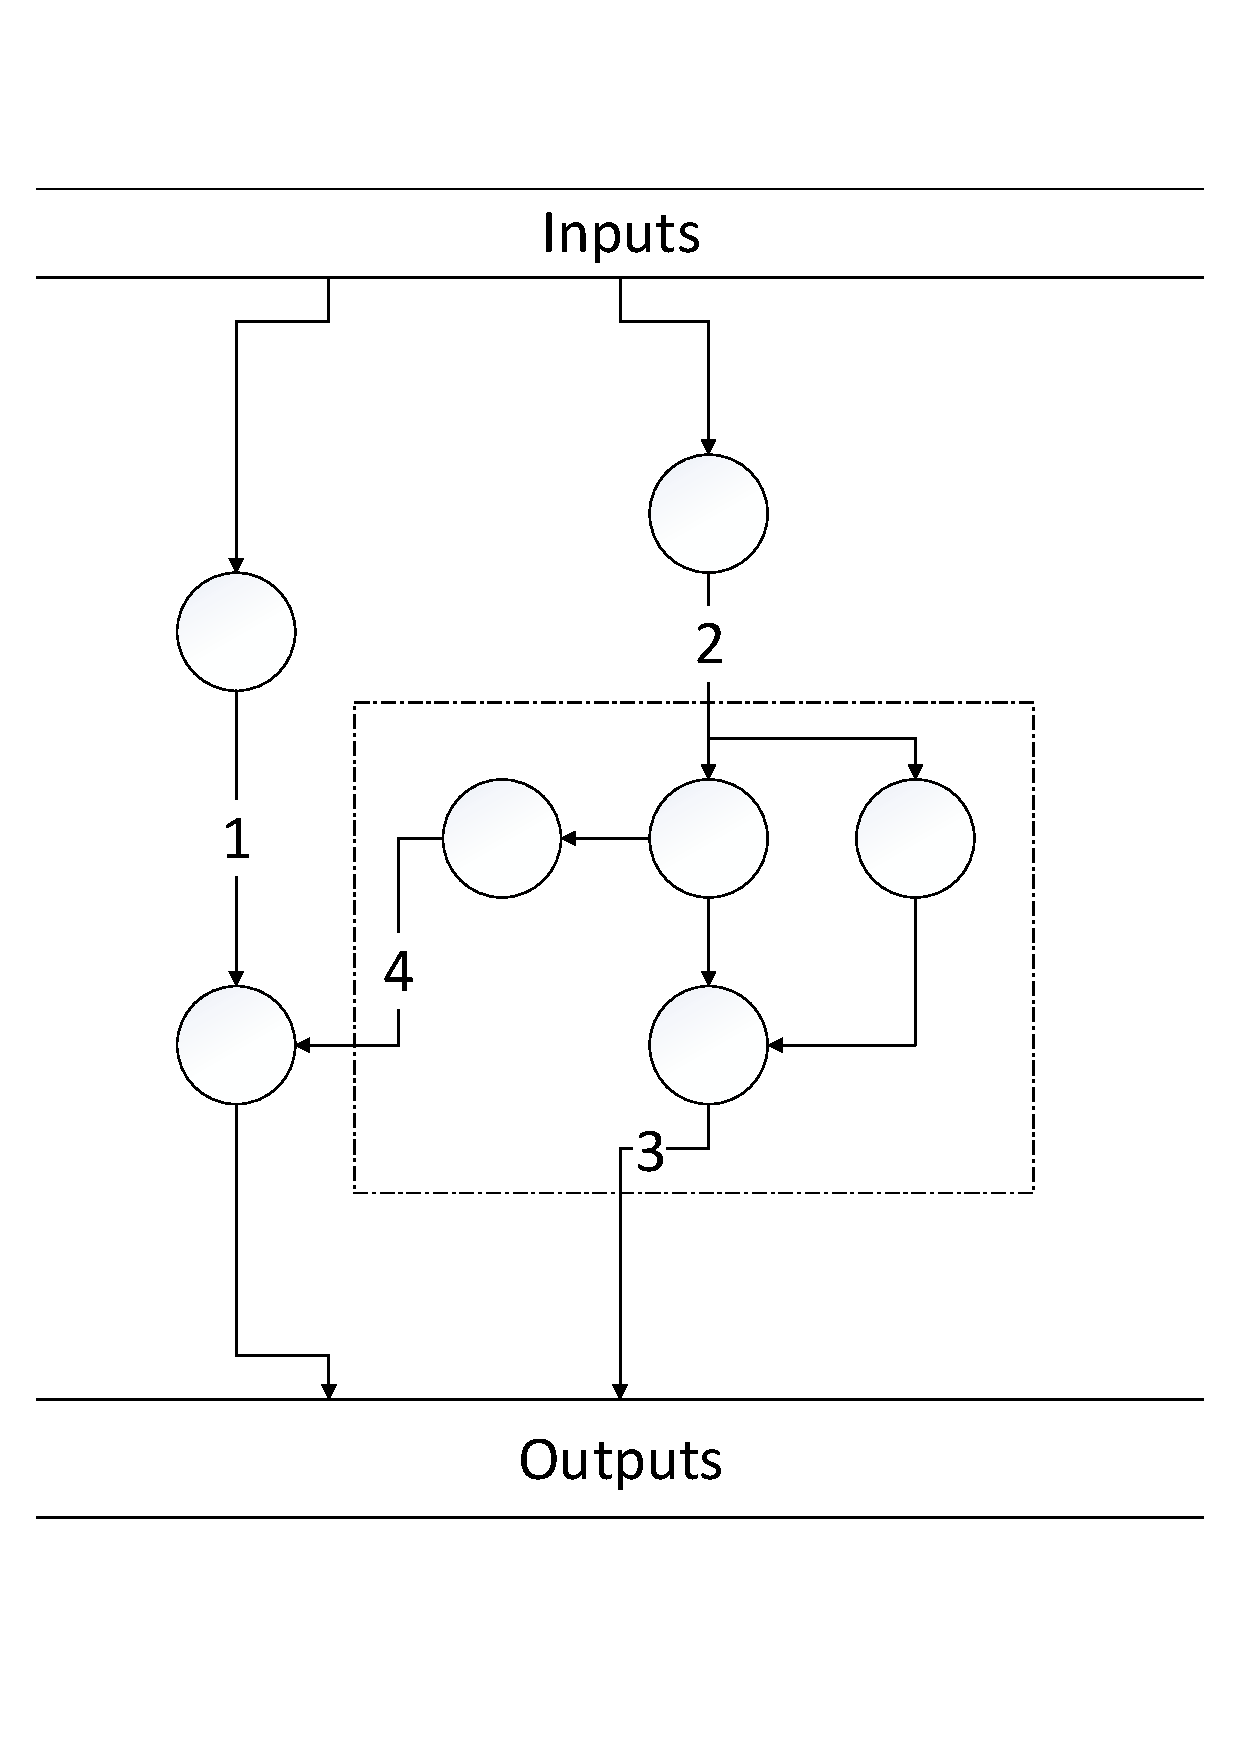
\includegraphics[width=\linewidth]{images/MakeIOList.pdf}
         \caption{MakeIOList} \label{imMakeiolist} 
      \end{center}

   \end{figure}
   We
   iterate through every signal in our partition. For each one we check if we
   have a source (line 3), if not it must be a primary input. Similarly, on
   line 7 we check if we have a sink which is not represented within our
   partition. If so, promote it to a primary output of the partition.

   So for example, in Figure \ref{imMakeiolist} signal 2 has no source within
   the partition, and so is promoted to primary input. Signal 3 and 4 both have
   outputs outside the partition, and so are promoted to primary outputs.


   \newpage 
   \subsection{RecoveryTime}
   For a given partition, calculate its
   error recovery time.  
   \begin{algorithm}

      \begin{center}


         \begin{tabularx}
            {\linewidth}{llX} \toprule Variable & Type &
            Description\\
            \midrule
            $partition$ & \textbf{Model} & The partition to calculate the recovery time for\\
            $numPartitions$ &\textbf{Integer } &  Estimated final number of partitions \\
            $clockPeriod$ & \textbf{Float} & Estimated clock period of final circuit\\$latency$ &\textbf{Float } &  Circuit
            latency (i.e. time for input to completely propagate to output) in
            seconds\\
            $clockPeriod$ &\textbf{Integer } & Estimated period of
            the final circuit, in seconds. This is estimated as $1.8\times$ the
            clock period of the original circuit\\
            $criticalPath$ &\textbf{Integer } &  Maximum number of steps between an input and an
            output\\
            $numFF$ &\textbf{Integer } &  Number of Latches in
            circuit\\
            $numLUT$ &\textbf{Integer } &  Number of look up tables
            in circuit\\
            $resynchronisationTime$ &\textbf{Float } &  Time, in
            seconds, that it takes to resynchronise circuit\\
            $detectionTime$
            &\textbf{Float } &  Time, in seconds, that it takes to detect an
            error\\
            $reconfigurationTime$ &\textbf{Float } &  Time, in
            seconds, that it takes to reconfigure circuit\\
            $communicationTime$
            &\textbf{Float } &  Time, in seconds, that it takes to transmit
            reconfiguration request to controller\\
            \bottomrule

         \end{tabularx}

      \end{center}
      \caption{RecoveryTime}\label{recoverytime}

      \begin{algorithmic}[1]
         \Procedure{RecoveryTime}{$partition, numPartitions, clockPeriod$} 
         \State
         $latency \gets clockPeriod\times{}(criticalpath+1)$ 
         \State
         $detectionTime \gets latency$ 
         \State $resynchronisationTime \gets
         latency$ 
         \State $reconfigurationTime \gets \mbox{max}(numFF,
         numLUT)/160\times 1.48^{-5}$ 
         \State $communicationTime \gets 5\times
         50\times(numPartitions+1)\times clockPeriod$ 
         \State $recoveryTime
         \gets
         detectionTime+resynchronisationTime+reconfigurationTime+communicationTime$

         \Return $recoveryTime$ \EndProcedure 
      \end{algorithmic}


   \end{algorithm}
   The derivation of this algorithm and the values used is
   fully discussed in Section \ref{secTMR}. The criticalpath is a measure of
   the maximum number of latches on a path from input to output. The +1 is to
   account for the contribution of combinational logic, which may be up to one
   additional clock cycle of latency. $numPartitions$ and $clockPeriod$ as passed to this function are calculated as per Section \ref{DesignEstimates}.


   \newpage 
   \subsection{AddNode}
   Insert a node into an existing partition, or
   circuit, while updating appropriate parameters (i.e. maximum path length and
   signals) which are depended upon by other components (i.e. recovery time
   calculation and \gls{DFG} traversal respectively).  Additionally, detect any
   newly created cycles and cut them.  This ensures that the circuit is always
   an acyclic graph with every node reachable.  
   \begin{algorithm}


      \begin{center}

         \begin{tabularx}
            {\linewidth}{llX} \toprule Variable & Type
            & Description\\
            \midrule $partition$ &\textbf{Model } &  Model
            containing DFG representing partition to add node to\\
            $node$
            &\textbf{BlifNode } &  Node to add\\
            $signal$ &\textbf{Signal
            } &  \\
            $signalName$ &\textbf{String } &  Name of a Signal\\

            $newName$ &\textbf{String } &  The new name of a Signal if and
            after it's been cut\\
            $partition.signals$ &\textbf{Map(String
               $\to$ Signal) } &  Map of signal name to Signal \\

            $signal.sinks$ &\textbf{List(BlifNode) } &  List of sinks for a
            Signal \\
            $signal.source$ &\textbf{BlifNode } &  Source, or
            driver, for a Signal \\
            $inCost$ &\textbf{Integer } &  Maximum
            number of critical path steps to reach node, not counting the node
            itself \\
            $explored$ &\textbf{Map(BlifNode $\to$ Boolean) } &
            Whether a node has been reached yet in the current iteration \\

            \bottomrule 
         \end{tabularx}

      \end{center}

      \caption{AddNode}\label{addnode} 
      \begin{algorithmic}[1]
         \Procedure{AddNode}{$partition, node$} 
         \State $nodes.insert(node)$
         \ForAll{$name \in node.inputs$} \If{IsRenamed($signalName$)} 
         \State
         $newName \gets$ GetNewName$(name)$ \Comment{If this signal has been
            renamed already to avoid a cycle, rename this occurrence of it.}

         \State Replace$(node.inputs, signalName, newName)$ \Comment{Replace
            the original name with what it was renamed to} 
         \State $signalName
         \gets newName$ \EndIf 
         \State $signal \gets
         partition.signals[signalName]$ 
         \State $signal.sinks.Add(node)$ \EndFor

         \State $signal \gets partition.signals[node.output]$ 
         \State
         $signal.source \gets node$


         \State $inCost \gets 0$ \ForAll{$signalName \in node.inputs$} 
         \State
         $signal \gets partition.signals[signalName]$ 
         \State $source \gets
         signal.source$ \If{$partition.costs[source] > inCost$} 
         \State $inCost
         \gets partition.costs[source]$ \EndIf \EndFor 
         \State
         UpdateCostsAndBreakCycles$(partition, node, NULL, node, inCost,
         explored, costs)$ \EndProcedure 
      \end{algorithmic}

   \end{algorithm}

   Lines 3-13 update the appropriate signals, adding the node as a source or
   sink to the relevant signals if they exist within the partition, or creating them implicitly if they don't already exist.
   Line 4 checks if the input signal referred to has been renamed by CutSignal in Algorithm \ref{algCutsignal}.
   If it has, retrieve the new name for the signal and rename the input signal accordingly.
   CutSignal only renames inputs, not outputs, thus this check only needs to be performed for circuit inputs.
   Lines 14-22 then update the maximum path length (or latency in
   clock cycles) while detecting and cutting any newly created cycles.


   \newpage 
   \subsection{UpdateCostsAndBreakCycles}
   Recursively traverse our
   network to update maximum path lengths to account for our new node and
   additional paths. While traversing the network, detect and break any cycles
   we encounter.  This turns a possibly cyclic \gls{DFG} with partially
   computed path lengths, into an acyclic \gls{DFG}---or \gls{DAG}---with fully computed path
   lengths.


   \begin{figure}

      \begin{center}

         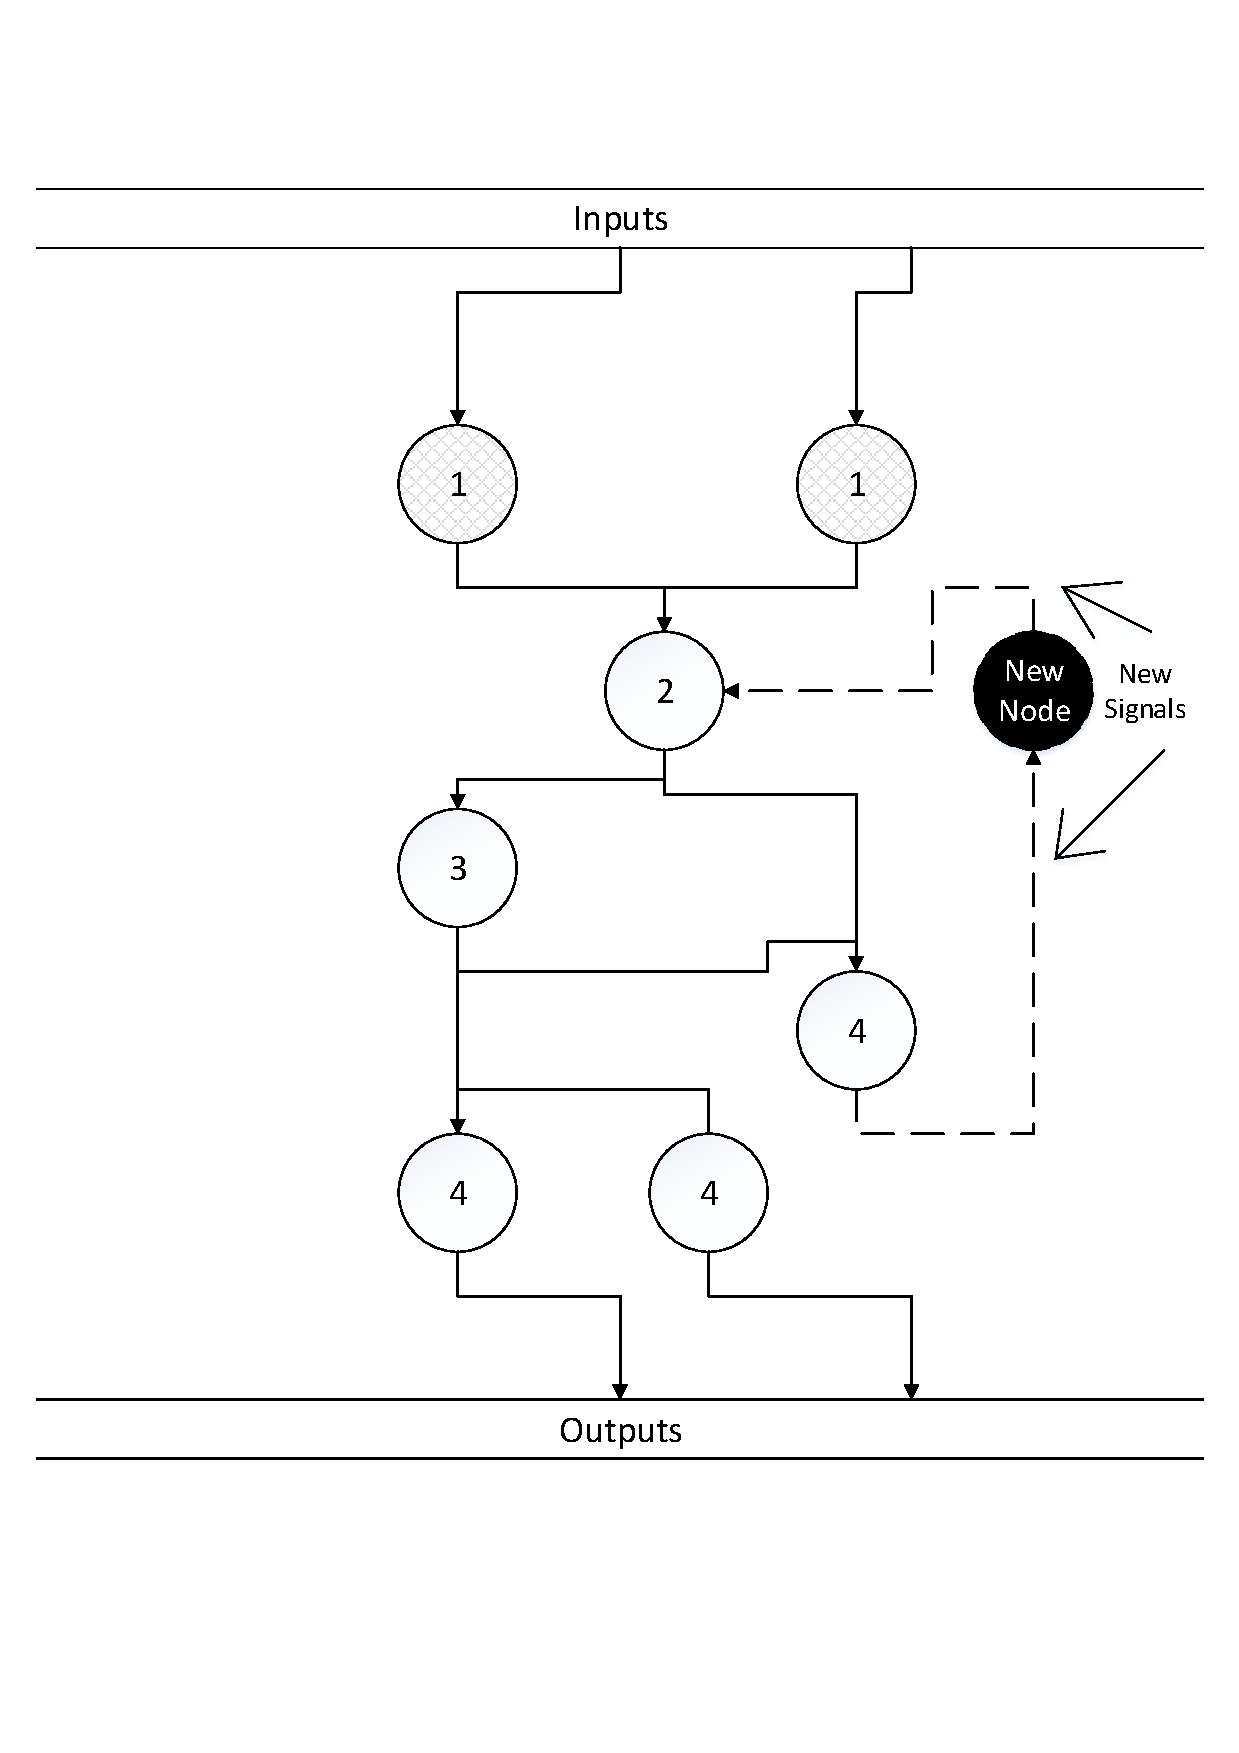
\includegraphics[width=\linewidth]{images/UpdateCostsAndBreakCycles.pdf}
         \caption{AddNode} \label{imAddnode} 
      \end{center}

   \end{figure}



   \begin{algorithm}

      \begin{center}

         \begin{tabularx}
            {\linewidth}{llX} \toprule
            Variable & Type & Description\\
            \midrule $partition$ &\textbf{Model } &  Model containing DFG representing partition to add
            node to\\
            $root$ &\textbf{BlifNode } &  Newly added node\\

            $parent$ &\textbf{BlifNode } &  Node we just came from\\

            $costToReach$ &\textbf{Integer } &  Maximum number of critical
            path steps to reach node, not counting the node itself \\

            $explored$ &\textbf{Map(BlifNode $\to$ Boolean) } &  Whether a
            node has been reached yet in the current iteration \\

            $partition.signals$ &\textbf{Map(String $\to$ Signal) } &  Map
            of signal name to Signal \\
            $parent.output$ &\textbf{String } &
            Name of the signal the parent nodes drives i.e. the signal we
            reached this node from\\
            $signal$ & \textbf{Signal } &  Signal we
            reached this node from\\
            $node.cost$ &\textbf{Integer } &  1 for
            latches, 0 for LUTs \\
            $costs$ &\textbf{Map(BlifNode $\to$
               Integer) } &  Map of the cost to reach each node \\
            $node$
            &\textbf{BlifNode } &  \\
            $signal.sinks$ &\textbf{List(BlifNode) } &  List of sinks for a Signal \\
            $cost$
            &\textbf{Integer } &  Number of critical path steps to reach node,
            including the node itself \\
            \bottomrule 
         \end{tabularx}


      \end{center}
      \caption{UpdateCostsAndBreakCycles}\label{updatecosts}

      \begin{algorithmic}[1]
         \Procedure{UpdateCostsAndBreakCycles}{$partition,
            root, parent, node, costToReach, explored$} \If{$explored[node] =
            true $ and $costs[node] \ge costToReach$} \Comment{No need to contnue down this path} 
        \Return \EndIf \If{$parent \neq
            NULL $ and $ node = root$} \Comment{We have a cycle}

         \State $signal \gets partition.signals[parent.output]$ \Comment{The
            signal edge we came in on} 
         \State CutSignal$(partition, signal)$

        \Return
        \EndIf 
         \State $cost \gets costToReach+node.cost$
         \If{$cost > costs[node]$} 
         \State $costs[node] = cost$ \Else 
         \State
         $cost = costs[node]$ \EndIf \ForAll{$child \in
            partition.signals[node.output].sinks$} 
         \State
         UpdateCostsAndBreakCycles$(partition, root, node, child, cost,
         explored)$ \EndFor 
         \State $explored[node] = true$ \EndProcedure

      \end{algorithmic}

   \end{algorithm}
   We care about two things. One, the
   maximum cost to reach a node, and two, detecting and removing any cycles.
   Given an existing \gls{DAG} which we insert a new node into, then

   \begin{enumerate}

      \item The new node is the root node of a subgraph within the \gls{DAG}.
      \item Nodes which are not within the subgraph cannot have the maximum
         cost to reach them change (as nothing has changed in any path to
         them).
      \item Any cycles must pass through the new node, as all the new edges are
         to or from the new node.
      \item Correspondingly, without any cycles the root node will only be
         reached once at the start.  
   \end{enumerate}
   Consider Figure
   \ref{imAddnode} where every node is a latch with cost to reach indicated.
   Our new node (filled in) is added to an existing \gls{DAG}. Our new node
   should now be the root of a subtree which includes all nodes reachable
   from our new node i.e. all nodes except those crosshatched which are
   unreachable from our new node.  We now traverse our \gls{DFG}
   recursively, updating the maximum cost to reach each node as we travel.
   Eventually, in our example we reach our newly added node again indicating
   a cycle. We thus cut the cycle as detailed in Algorithm
   \ref{algCutsignal}, recurse back a step,
   and continue until the entire \gls{DFG} has been traversed, at which
   point all cycles have been cut, and all nodes have the maximum path
   length to them updated.
   
   Using this information we develop our traversal
   algorithm.  Line 2 demonstrates an optimisation, in that once a path has
   been checked we need not recheck it unless we have found a more expensive
   path to it as otherwise nothing will change.  Lines 5-9 check if we have
   detected a cycle. If so, cut it through cutting the signal, which splits
   the signal into two: A primary output with the same source, and a primary
   input with the same sinks, as detailed further in Algorithm
   \ref{algCutsignal}.

   \newpage 
   \subsection{CutSignal}
   \label{cutsignal}
   Given a signal, cut it by
   splitting it into two signals, of which one is a newly named primary input
   with the same sinks as the cut signal had, and the other of which is a
   primary output with the same source and name as the original signal.
   Figure \ref{imCutSignal} demonstrates this transformation in action.

   \begin{figure}

      \begin{center}

         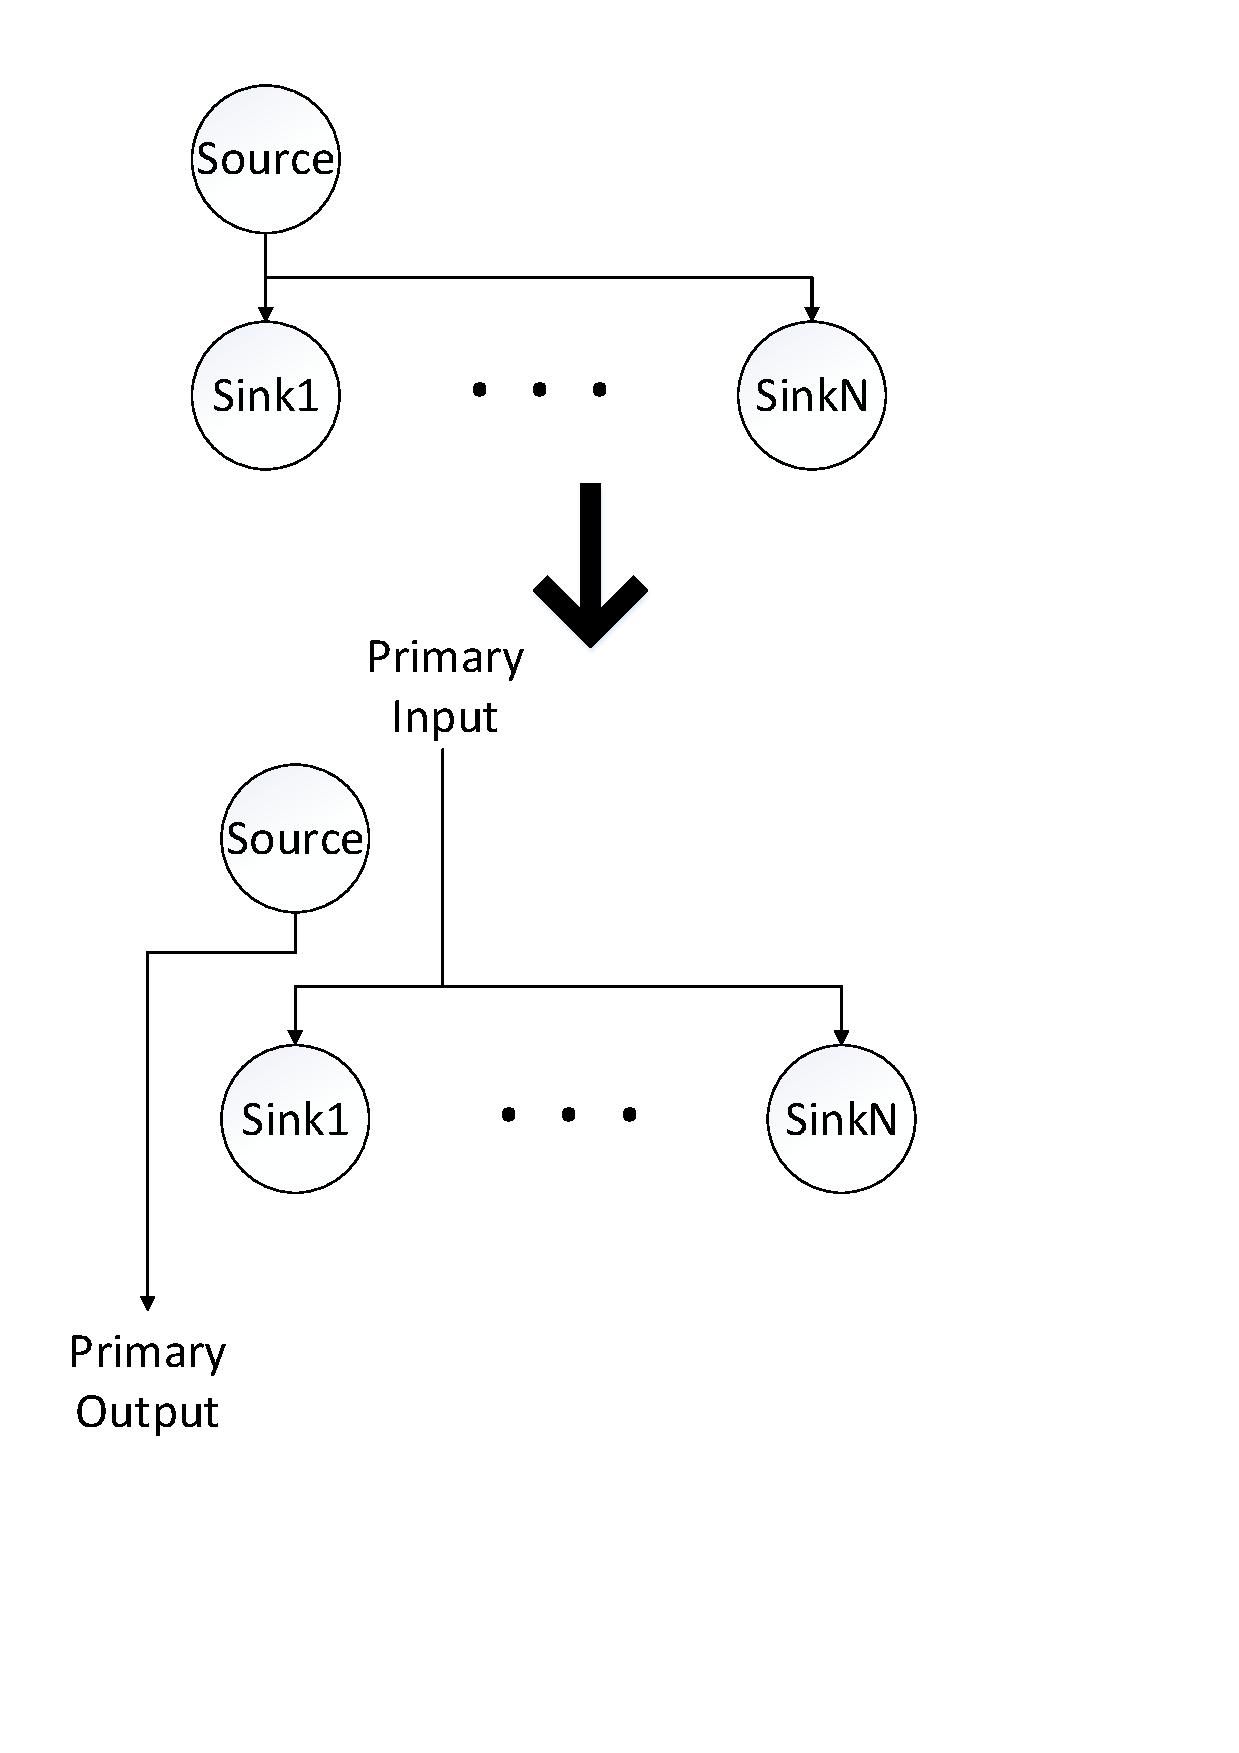
\includegraphics[width=\linewidth]{images/CutSignal.pdf}
         \caption{CutSignal} \label{imCutSignal} 
      \end{center}

   \end{figure}
   \begin{algorithm}

      \begin{center}

         \begin{tabularx}
            {\linewidth}{llX} \toprule
            Variable & Type & Description\\
            \midrule
            partition & \textbf{Model} & Model containing DFG representing partition to cut signal within \\
            signall & \textbf{Signal} & Signal to cut \\
            newInputSignal & \textbf{Signal} & New primary input signal with the sinks of the original\\
            newOutputSignal & \textbf{Signal} & New primary Output signal with the source of the original\\
            \bottomrule 
         \end{tabularx}


      \end{center}
      \caption{CutSignal}\label{algCutsignal}

      \begin{algorithmic}[1]
      	\Procedure{CutSignal}{$partition, signal$}
      		\State $newInputSignal \gets new Signal()$
      		\State $newInputSignal.source \gets NULL$
      		\State $newInputSignal.sinks \gets signal.sinks$
      		\State $newInputSignal.name \gets MakeNewName(signal.name)$ \Comment{Create a unique signal name through a reversible transformation}
      		\State $newOutputSignal \gets new Signal()$
      		\State $newOutputSignal.source \gets signal.source$
      		\State $newOutputSignal.sinks \gets new List$ \Comment{No inputs, so assign an empty list}
      		\State $newOutputSignal.name \gets signal.name$
      		\State $partition.signals[newInputSignal.name] \gets newInputSignal$
      		\State $partition.signals[newOutputSignal.name] \gets newOutputSignal$
      		\State
      		\ForAll{$node \in signal.sinks$}
      			\State replace$(node.inputs, signal.name, newInputSignal.name)$ \Comment{Replace input signal names in nodes with the new signal name}
		\EndFor
\EndProcedure
      \end{algorithmic}
      \end{algorithm}
      Lines 2-5 create a new primary input. It has no source (as it is a primary input of the partition) and the sinks of the original signal.
      Line 5 generates a new globally unique name for this signal which can be reversed to give the original signal name. In our implementation we prepend a constant string ``qqrin'' and specify that signal names of this form are reserved, as no benchmarks used signal names in that format.
      Lines 6-9 create a new primary output. It has no sinks and the source of the original signal. This signal retains the same name as the original signal.
      Lines 10-14 update all references to the old signal to refer to the appropriate new signal.


\newpage

   \subsection{Triplicate}
   \label{algTriplicate} Given a file containing a
   partition, read it in as a black box, triplicate it, add voter logic and
   write it back out to file.

   This method operates on the \gls{BLIF} in a low level way, dealing with
   manipulating the actual file contents, rather than operating on an abstract
   circuit representation, as we transform a flat circuit into a heirarchical
   circuit, in which our original flat circuit remains untouched but we insert
   voting and similar logic around it.
   
   This is done through reading in the circuit, instantiating three copies of it,
   and inserting these copies into a template which includes a voter circuit.
   We then generate the appropriate signals to connect the circuit inputs to each of the three identical partitions, the partition outputs to the voter,
   and the voter output to the circuit output.
   This new circuit is then written back out to file.
   Figure \ref{imTriplicate} represents this process graphically.


   \begin{figure}

      \begin{center}

         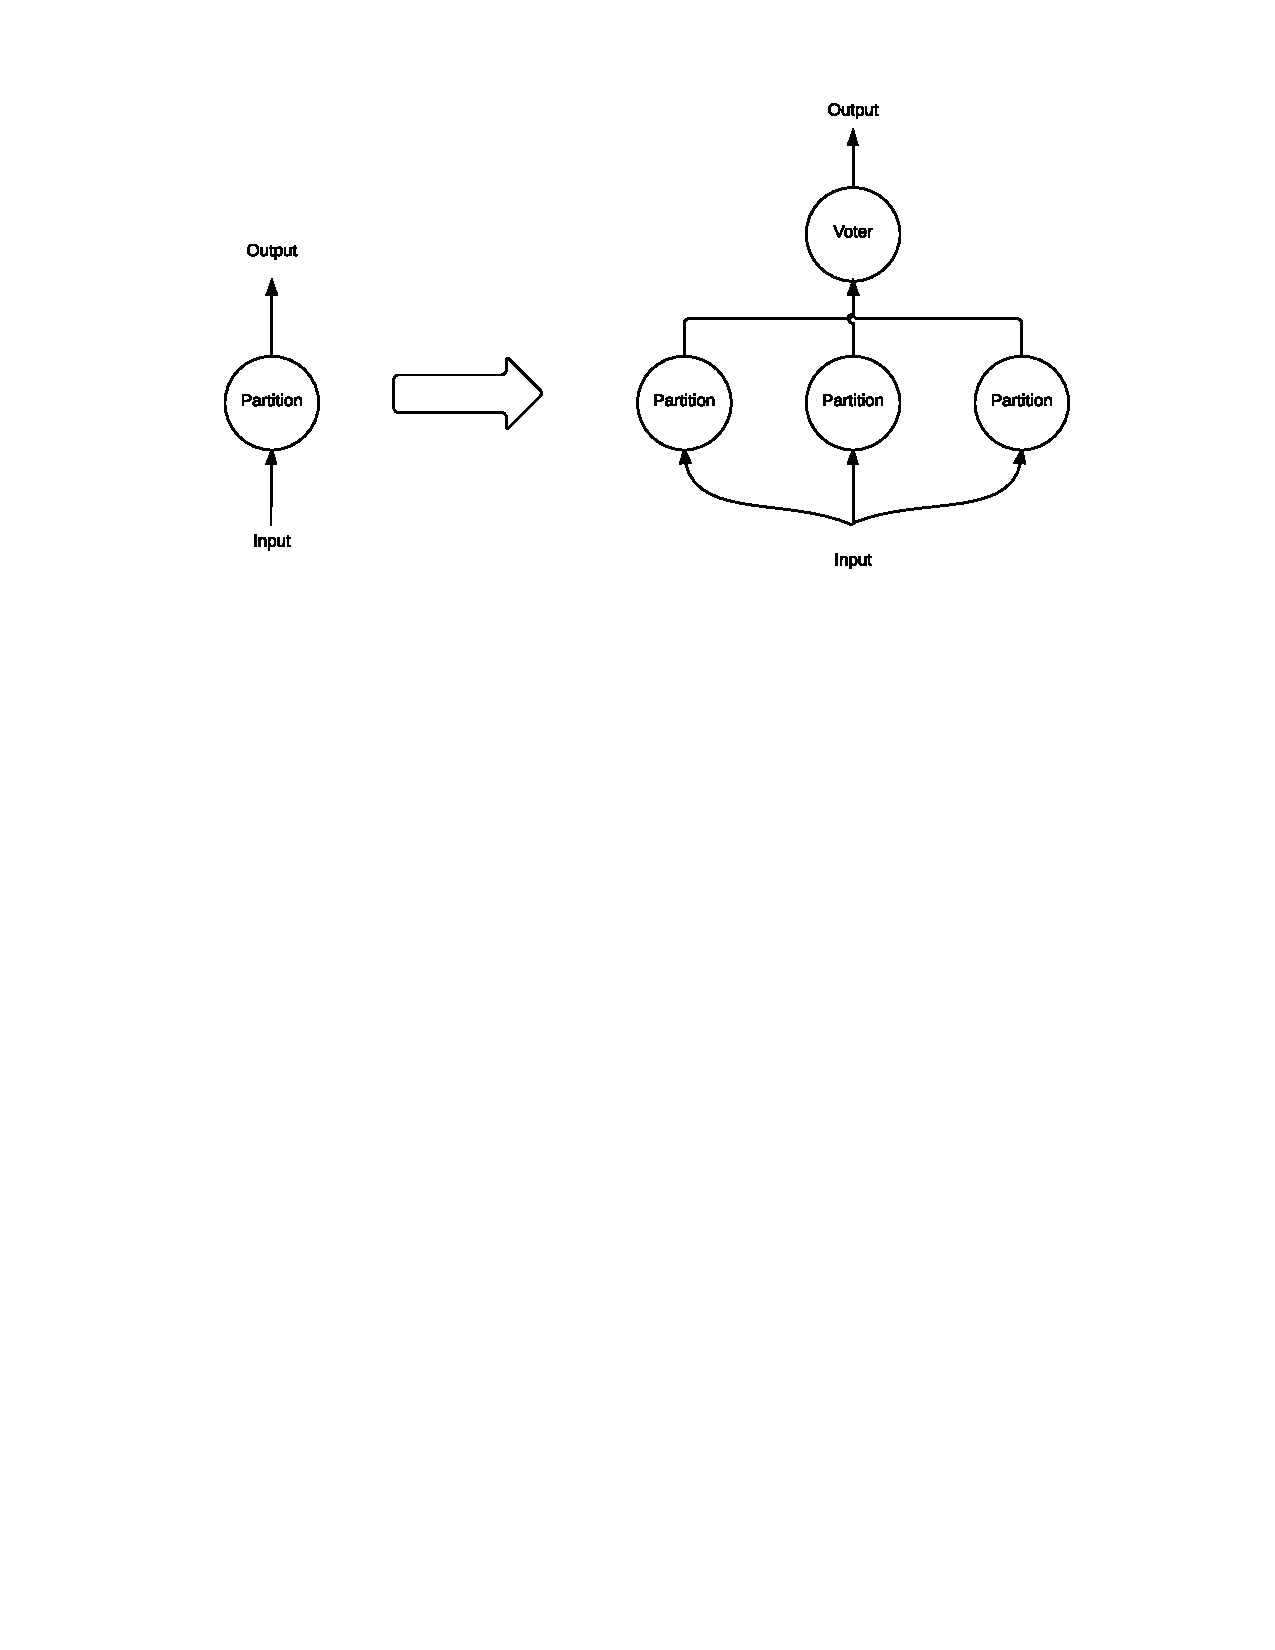
\includegraphics[width=\linewidth]{images/Triplicate.pdf}
         \caption{Triplicate} \label{imTriplicate} 
      \end{center}

   \end{figure}

   \newpage 
   \subsection{Join}
   \label{algJoin} Given a list of blif files,
   joins them all together into one circuit.
   Figure \ref{imMerge} represents the transformation graphically.
   
   This is accomplished through reading in each circuit from the input files, and instantiating each of these circuits as a black box subcircuit in a heirarchical design.
   The top level circuit is created with the same inputs and outputs as the original circuit, and contains a reference to each subcircuit.
   The inputs and outputs from each circuit are promoted up to the top circuit level, and all signals with same same name are tied together.
   As signal names are required to be globally unique, and are preserved through the partitioning process (recall that while cutting signals renames them, these renamed signals are internal to a set of triplicated partition and voter and thus not visible to the top level circuit) this then joins all the subcircuits up correctly, and to the appropriate circuit primary inputs and outputs.
   This process is representing graphically in Figure \ref{imJoin}.
   \begin{figure}

      \begin{center}

         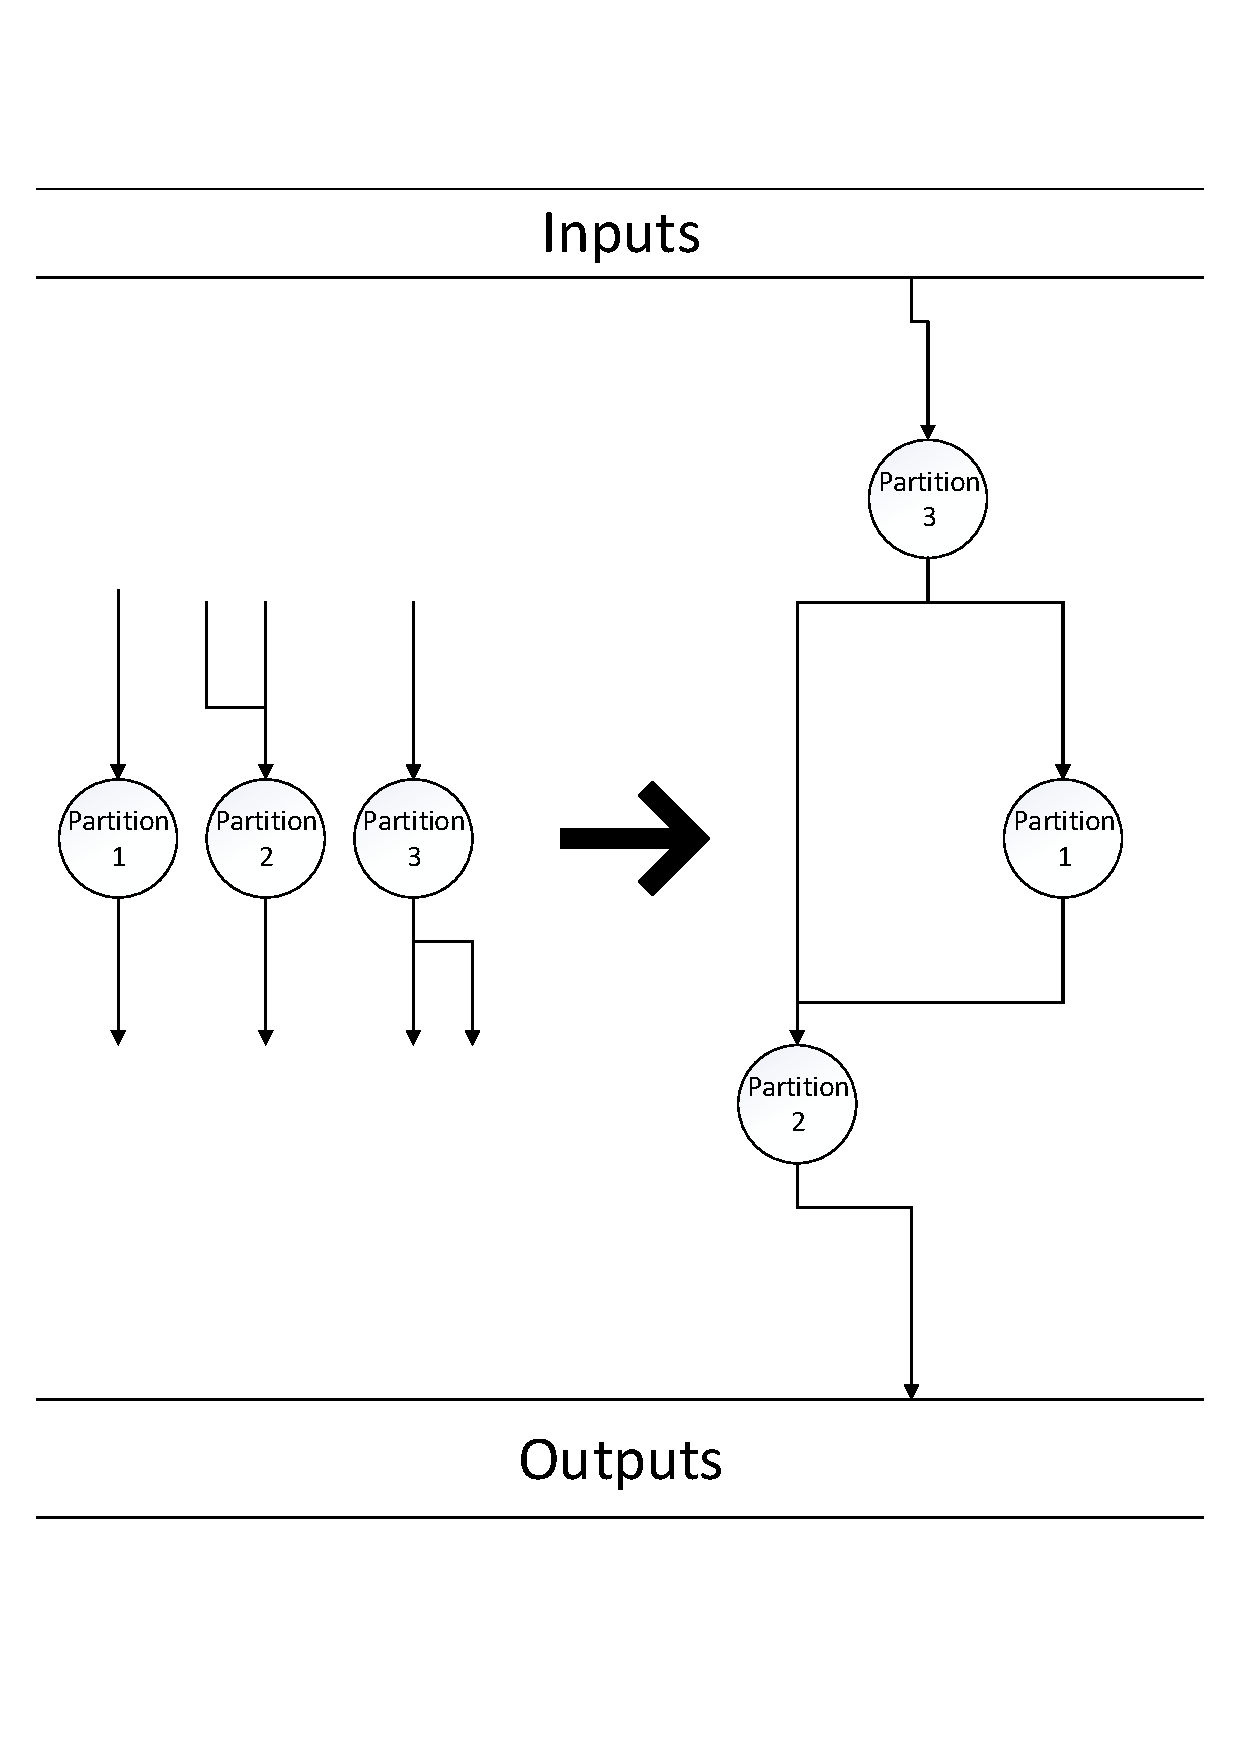
\includegraphics[width=\linewidth]{images/merge.pdf} \caption{Join high level overview}
         \label{imMerge} 
      \end{center}

   \end{figure}
   \begin{figure}

      \begin{center}

         \includegraphics*[viewport=500 230 1200 800,width=\linewidth]{images/Join.pdf}
         \caption{Joining Signals} \label{imJoin} 
      \end{center}

   \end{figure}


   \newpage 
   \subsection{Flatten}
   \label{algFlatten} Given a
   heirarchical \gls{BLIF} file, run it through
   \gls{ABC} to flatten it, and postprocess if
   necessary.  
   \begin{algorithm}

      \begin{center}


         \begin{tabularx}
            {\linewidth}{llX} \toprule Variable & Type &
            Description\\
            \midrule $file$ &\textbf{File } &  File to
            flatten\\
            $clockInfo$ & \textbf{List(String)} & List of latch parameters, including clock name, etc\\
            \bottomrule 
         \end{tabularx}

      \end{center}

      \caption{Flatten}\label{Flatten} 
      \begin{algorithmic}
         [1]
         \Procedure{Flatten}{$file$}
         \State \texttt{./abc -o output -c echo file}
         \State $clockInfo \gets $split(\texttt{grep -m 1 `.latch' file})
         \If{$clockInfo$} 
         \State $\texttt{sed -ri `s/(\textbackslash.latch.+)(2)/\textbackslash1 '} + clockInfo[3] + \texttt{` '} +
         clockInfo[4] + \texttt{` 2/' output} $\EndIf \EndProcedure 
      \end{algorithmic}


   \end{algorithm}

   By default \gls{ABC} flattens input files but performs no other optimisations, therefore we can call
   \texttt{./abc -o output -c echo input} to read in \texttt{input}, flatten it, and write it to \texttt{output}.
   Unfortunately, there exists a bug in \gls{ABC} where clock information is stripped from latches.
   To circumvent this we require that all latches have the same clock information (clock name, trigger, initial state),
   which holds for all of the twenty largest \gls{MCNC} benchmarks,
   and then use grep and sed to extract the clock information from the original circuit and edit it back into the flattened circuit.


   \subsection{Test}
   \label{algTest} \gls{ABC} is also used to optionally test
   the generated circuit to verify that it is equivalent to the original. It
   does this by creating a miter circuit, which is derived by pairing inputs
   for the two circuits, and feeding output pairs into an XOR gate which are
   then OR'd to produce the single output. For any given input, the miter
   circuit output is 0 if both circuits produce the same set of outputs for the
   input set, and 1 if the outputs differ, which turns verification into a
   \gls{SAT}.  The circuits are then simplified by merging equivalent nodes,
   removing redundant logic and testing inputs.
   This proceeds until a counter example is found, or the circuit is shown to
   have constant output 0 for all possible inputs \cite{abcSEC, abcCEC}.  While
   solving a \gls{SAT} is NP-complete, in practice the large amount of
   redundancy in \gls{TMR}'d circuits allows testing to complete in only a few
   seconds for the twenty largest \gls{MCNC} benchmarks.


   \section{Performance}
   The algorithm must visit each node in the input
   circuit once to add it to a partition, giving a factor of $n$.
   Additionally, for each node added to a partition, in the worst case every
   other node already in the partition must be visited to detect cycles and
   update costs, making AddNode worst case linear in the number of nodes in the
   partition.  Constructing the list of inputs and outputs takes time
   proportional to the number of signals in the partition. In practice, the
   number of signals will be approximately equal to the number of nodes (each
   node drives one signal, plus the number of inputs to the circuit).  This
   gives us worst case $O(n^2)$.
   
   Note that this does not include the contribution from rerunning the partitioner as we update our estimate for the number of partitions.
   This depends on the maximum number of partitions (as the estimate can only be revised upwards) which is a function of the number of circuit elements,
   giving worst case of at most $O(n^3)$. \fxnote{Expand}
   
   
   Triplicating is linear in the number of
   inputs and outputs, joining is $O(nk)$ where n is the number of circuits,
   and k is the number of inputs and outputs for each circuit. \fxnote{Check.
      Is this just linear in number of IOs?} In practice, for the twenty
   largest \gls{MCNC} benchmark circuits each step is sub-second
   compared to \gls{VPR}'s running time of up to an hour for some \gls{TMR}'d
   benchmark circuits, as outlined in Section \ref{timing}.


   \section{Correctness}\label{secTesting}
   A threefold approach to verifying the correctness of
   the implementation was taken.  Firstly, small sample circuits were
   partitioned and the resulting circuits were examined manually to verify
   correct operation. Manual verification is, however, not practical for all
   but the smallest circuits so the small sample circuits were generally just
   used to test specific corner cases, while two other methods were used to
   check the benchmarks. As detailed earlier in this section, \gls{ABC} was
   used to verify that the generated circuits were functionally equivalent.
   That is to say, for any set of inputs both the original and TMR'd circuit
   had identical outputs.  Next, circuit properties such as number of elements
   could be examined and compared to expected results, as is done in Section
   \ref{resSanity}.  One additional incidental test was verification that the
   generated file is a valid \gls{BLIF} file. \gls{VPR} and \gls{ABC} are both
   quite picky and generally either error out or crash on circuits which don't
   exactly match the expected format.



   \section{Design Choices}
   As much as possible, we would like our
   implementation to be easily extensible to multiple architectures. The actual
   partitioner operates on a \gls{DFG} so it can be mostly architecture
   agnostic, only requiring the estimation functions to be architecture aware.
   From initial steps in this thesis we wrote Python scripts capable of
   performing basic operations on \gls{BLIF} files which were used as the basis
   for Triplicating and Joining. Given time the functionality of each step
   (partition, triplicate, etc) could all be combined in one program; however
   it was considered a much lower priority than creating a working reference
   implementation.

   Other design choices include deciding on \gls{VPR} due to its open nature as
   discussed earlier in Section \ref{VPRSection}, and how we traverse our
   \gls{DFG}. A depth-first traversal as we ended up using tends to generate
   long narrow pipelines within each partition, thus increasing the number of
   register stages but reducing the number of inputs and outputs for each
   partition, whereas a breadth-first traversal lends itself to fewer register
   stages for the same number of nodes but more inputs and outputs (and hence
   voters) for each partition. Benchmark results
   comparing the two options can be found in Section \ref{bfs}.
    A possible future improvement is implementing a
   more advanced traversal algorithm, for example A* with an appropriate
   heuristic could allow for more elements per partition.

   Additionally, we are faced with a choice as to when in the \gls{CAD} process
   to partition. The closer to the end of the process the more control we have,
   and the better our ability to estimate area and timing, but the harder it is
   to partition. As we are inserting new elements we want to partition before
   packing/placement to allow \gls{VPR} to pack and place our inserted
   elements.

   \subsubsection{Choice of Language} We have used a combination of languages,
   mainly Python and C++. Language choice primarily came down to preference
   regarding familiarity and personal taste although a few other considerations
   were kept in mind.  For \gls{BLIF} joining and insertion of the voting logic
   Python was used. \gls{BLIF} files are plain text and the text parsing to
   join and insert is computationally simple, so the primary concern was short
   development time while still being readable and maintainable (although
   Python's performance on text is still quite
   reasonable)\cite{LanguageBenchmark}.  For the actual partitioner C++ was
   chosen for a few reasons. Firstly, it was expected that the area and time
   estimations could be quite computationally expensive, so a lower level
   compiled language was chosen for performance
   reasons\cite{LanguageBenchmark}. Secondly, \gls{VPR} is written in C, so
   using C or C++ allowed for easy code reuse, or merging the partitioner and
   \gls{VPR}. Our reason for choosing C++ over C was that we preferred an
   object oriented language as we felt it would be easier to maintain, and
   would better lend itself to our goal of extensibility, as well as its
   libraries making our implementation much easier.


   \section{Input File Format}
   \label{secBlif} The \gls{BLIF} file format is a
   textual format which describes an arbitrary sequential or combinational
   network of logic functions\cite{BLIF}.  Our partitioner only supports a
   subset of the \gls{BLIF} specification, specifically only those elements
   supported by \gls{VPR} and used in our benchmark files.
   A sample \gls{BLIF} file is included in Listing \ref{SampleBlif} and 
   Table \ref{BLIFCommands} lists the supported commands and their meanings.
\begin{table}
      \begin{center}
   \begin{lstlisting}[caption=BLIF file layout, label=SampleBlif]
   .model voter
      .inputs in1 in2 in3
      .outputs out1 out 2
      .clock clock
      .names in1 in2 in3 out1
      11- 1
      1-1 1
      -11 1
      .latch in1 out2 re clock 1
      ...  
      commands 
      ...  
      .end
   \end{lstlisting}
\end{center}\end{table}


\begin{table}
      \begin{center}
   \begin{tabular}
      {lll} Model name: & .model $\langle$Name$\rangle$ & The name
      of the model.\\
      Input List: & .inputs \{SignalName\} & The model inputs.\\

      Output List:& .outputs \{SignalName\} & The model outputs.\\
      Clock List: &
      .clock \{SignalName\} & The model clocks.\\

      \multicolumn{2}{l}{\gls{LUT}:} & .names \{InputSignals\}
      $\langle$OutputSignal$\rangle$\\
      &&\{Line\}\\
      \multicolumn{2}{l}{Latch:}
      & .latch $\langle$InputSignal$\rangle$ $\langle$OutputSignal$\rangle$
      [Trigger ClockSignal] [InitialState]\\
      \multicolumn{2}{l}{Optional End Marker:} &
      .end 
   \end{tabular}
   \caption{\gls{BLIF} commands}\label{BLIFCommands}
\end{center}\end{table}


   \{Name\} indicates 1 or more of Name. $\langle$Name$\rangle$ indicates a
   compulsory field. [Name] indicates an optional field.  A combinational logic
   element (.name) is followed by one or more lines describing the logic
   function it implements. However, our partitioner only cares about node type
   and the signal names (named with SignalName above) as it builds and traverses the
   \gls{DFG}. All other element information is stored and written back out when
   the node is written.

   \gls{VPR} only supports flat \gls{BLIF} files, so only one module
   declaration is allowed per \gls{BLIF} file. \gls{ABC} can be used to flatten
   \gls{BLIF} files for use by \gls{VPR}.




   \chapter{Results}\label{results}

   \section{Benchmarking Procedure}
   These results were
   collected by running benchmark circuits through an automated test suite
   written in Python by the author. For each benchmark circuit, and each target
   recovery time, a minimum of 15 repetitions were performed to average out the variability
   in results due to the stochastic nature of \gls{VPR}'s placement algorithm.
   The original circuit was run through \gls{VPR} to collect base results, then the
   circuit run through our partitioner to \gls{TMR} it. The \gls{TMR}'d version was then
   verified by \gls{ABC} to check its functional equivalence to the original,
   and then run through \gls{VPR} to collect \gls{TMR}'d results. Each run of \gls{VPR} used a
   randomly generated seed for the placer.  The mean of the reported values
   across all successful runs was recorded.  The benchmarks used were the 20
   largest \gls{MCNC} LGSynth93 circuits technology mapped to flip-flops and 4-input \glspl{LUT}, as provided by the open-source
   \gls{VTR} project\footnote{v1.0: \url{http://code.google.com/p/vtr-verilog-to-routing/}} and described in table
   \ref{benchmarkList}.
   As the number of \glspl{LUT} is larger than the number of latches for all twenty \gls{MCNC} circuits we used, the number of \glspl{BLE} is equal to the number of \glspl{LUT}.
    The set of target recovery times used were $10^{-3},
   2.5\times10^{-4}$, $1.2\times10^{-4}$ and $7.5\times10^{-5}$s.  The voter used is a simple
   3-input \gls{LUT}, which uses one \gls{BLE} per output signal from each
   partition.
   Table \ref{Results1e-3} in the Appendix, where each circuit had only one partition, contains equivalent values for area overhead and clock slowdown as if a 
   more traditional \gls{TMR} approach were used, which simply triplicated the entire circuit allowing our approach the be compared.

   \begin{table}

      \begin{center}

         \begin{tabular}
            {lrrrr} \toprule &
            \multicolumn{4}{c}{Number of:}\\
            \cmidrule{2-5} Name & Inputs &
            Outputs & Latches & \glspl{LUT}\\
            \midrule
alu4 & 14 & 8 & 0 & 1522\\
apex2 & 38 & 3 & 0 & 1878\\
apex4 & 9 & 19 & 0 & 1262\\
bigkey & 229 & 197 & 224 & 1707\\
clma & 62 & 82 & 33 & 8381\\
des & 256 & 245 & 0 & 1591\\
diffeq & 64 & 39 & 455 & 1494\\
dsip & 229 & 197 & 224 & 1370\\
elliptic & 131 & 114 & 1218 & 3602\\
ex1010 & 10 & 10 & 0 & 4598\\
ex5p & 8 & 63 & 0 & 1064\\
frisc & 20 & 116 & 924 & 3539\\
misex3 & 14 & 14 & 0 & 1397\\
pdc & 16 & 40 & 0 & 4575\\
s298 & 4 & 6 & 8 & 1930\\
s38417 & 29 & 106 & 1463 & 6096\\
s38584.1 & 38 & 304 & 1260 & 6281\\
seq & 41 & 35 & 0 & 1750\\
spla & 16 & 46 & 0 & 3690\\
tseng & 52 & 122 & 385 & 1046\\
            \bottomrule 
         \end{tabular}
         \caption{Benchmark
            circuits used} \label{benchmarkList} 


   \end{center}\end{table}\subsection{Target
      Architecture} 
   \begin{figure}

      \begin{center}

         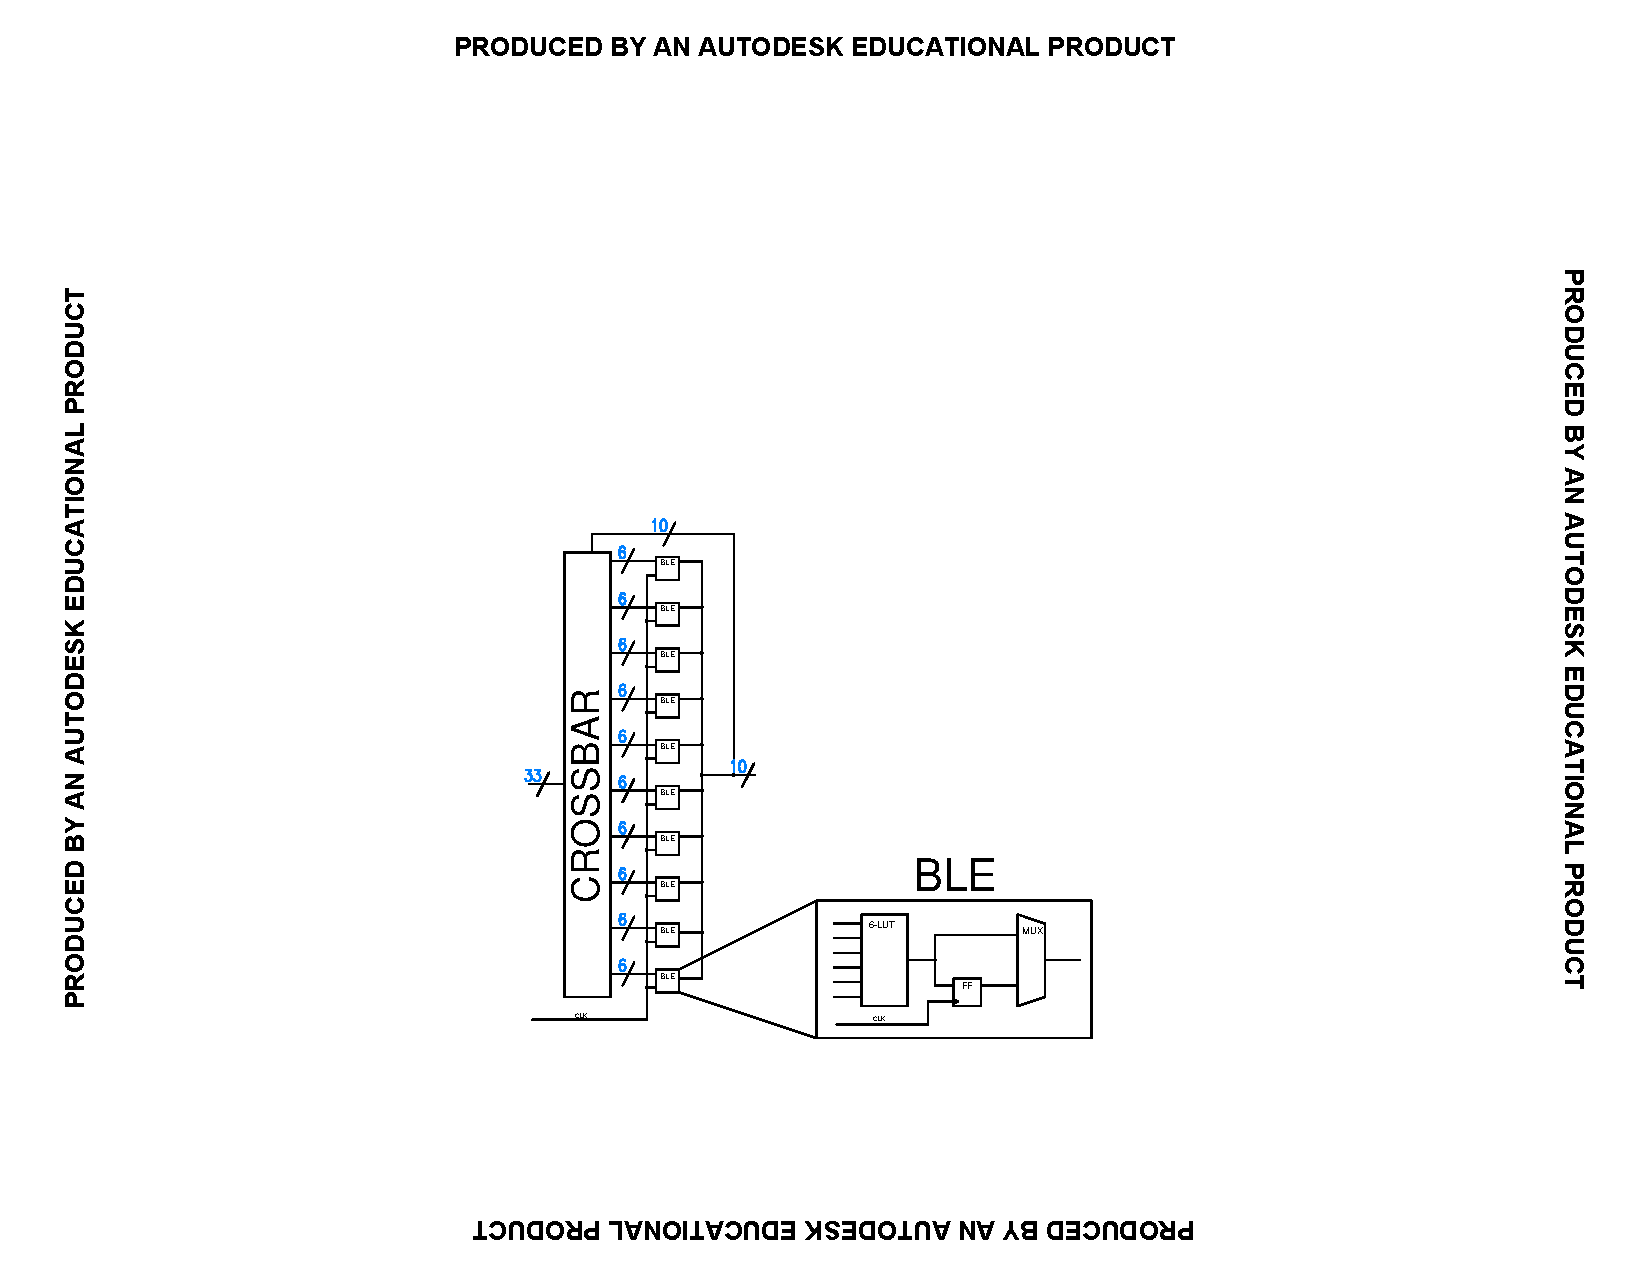
\includegraphics[clip,trim=8cm 4cm 8cm 8cm]{images/CLB.pdf}
         \caption{\gls{CLB} Architecture} \label{ArchFig} 
      \end{center}


   \end{figure}
   \gls{VPR} allows us to specify a custom architecture for it to
   run against in an XML format. We opted for the default architecture detailed
   in \cite{VPRManual} consisting of a grid of \glspl{CLB} each consisting of
   ten fully interconnected \glspl{BLE}, and each \gls{BLE} having a latch and
   6-\gls{LUT} as ilustrated in Figure \ref{ArchFig}.  Table \ref{ArchTab}
   details the number of primitives (latches and \glspl{LUT} per \gls{CLB}.
   Primarily of interest is that each \gls{BLE} has 6 inputs and 1 output and
   each \gls{CLB} has 33 inputs and 10 outputs.
   
   Our architecture consists of 6-input \glspl{LUT} while our design has \glspl{LUT} with fewer inputs so there is potential for multiple \glspl{LUT} to be packed into one.
   \gls{VPR} does not optimise in this way, instead relying on \gls{ABC} for optimisation.
   To confirm this we compared our results to a small set conducted on a similar architecture with 4-input \glspl{LUT} and found that there while there were slight ($\approx1\%$) differences in running time and variations between the packed netlist, for the same seed the the final circuit area and clock period are identical.


   \ctable[ botcap, caption = Architecture Elements, label = ArchTab ]{llll}{
   }{ \FL Component & Number & Notes\ML Flip Flop & 1 per BLE& Shown as FF on
      Diagram\NN 6-LUT & 1 per BLE & \NN MUX & 1 per BLE \NN BLE & 10 per CLB
      &\NN Crossbar & 1 per CLB &\NN CLB & Autosized by VPR & \LL }



   \section{Sanity Check}
   \label{resSanity} The following results are for the
   tseng.blif circuit at a target recovery time of $7.5\times10^{-5}$s. The reported
   values can be compared to each other as a manual sanity check allowing for
   additional confirmation of the correct operation of the partitioner.

   We are able to confirm all the values which should add up, do. For example:
   \begin{eqnarray*}
      LUTsTMR &=& 3\times LutsBase + \sum PartitionOutputs\\
      3730 &=& 3\times1046 + 305 + 287\\
      3730 &=& 3730\\
      LatchesTMR &=&  3\times LatchesBase\\
      1155 &=& 3\times385\\
      NumNodes &=& \sum LUTs+\sum Latches = LUTsBase+LatchesBase \\
      1431 &=& 640+406+206+179 = 1046+385\\
      1431 &=& 1046 + 385 = 1431\\
      PartitionOutputs &>& CutLoops\\
      RecoveryTime &=&
      ClockPeriod\times CriticalPath\times 2 + 250\times(NumPartitions+1)\times
      ClockPeriod + \\
      & &ClockPeriod\times \left\lceil
      \frac{NumBLEs}{160}\right\rceil\times 1.48\times10^{-5}\\
      &=&
      10.9\times10^{-9}(2\times20+750)+4\times1.48\times10^{-5}\\
      &=&
      8.649\times10^{-6}+5.92\times10^{-5}\\
      &=& 6.78\times10^{-5}
   \end{eqnarray*}
   $LUTs$ and $Latches$ refers to per partition numbers of \glspl{LUT} and latches respectively. $LUTsBase$ and $LatchesBase$ refer to numbers for the entire circuit.
   $PartitionOutputs$ is the number of voted-on outputs from each partition and is equal to the number of feedforward edges (edges into another partition, or primary outputs from the circuit) and the number of feedback edges, or edges reused within the partition. $CutLoops$ is the number of cut loops on a per-partition basis and is the same as the number of feedback edges. Where a signal is used part of a voted-on cycle (feedback) and in another partition (feedforward) it is only counted once, not twice.
   $ClockPeriod$ is the estimated clock period and $NumPartitions$ is the number of partitions.
   
    In Table \ref{tabSanityPartitions}
   Outputs is the number of feedforward edges (signals going to other
   partitions) $+$ the number of feedback edges (cut cycles). Some other observations
   from this data: Our estimated clock period was conservative. We estimated
   10.9ns when the circuit actually came in at 8.9ns.  \gls{VPR} takes much
   longer on triplicated circuits than on the original. 6 times longer in this
   example.  
   \begin{table}
      \begin{center}

      \begin{tabular}
         {lr} \toprule File & tseng.blif\\

         Number of Nodes & 1431\\
         Estimated Latency (ns)& 10.9\\
         Partitions &
         2\\
         Number of Inputs Base & 52\\
         Number of Inputs TMR & 52\\
         Number of
         Outputs Base & 122\\
         Number of Outputs TMR & 122\\
         Number of LUTs Base
         & 1046\\
         Number of LUTs TMR & 3730\\
         Number of Latches Base & 385\\

         Number of Latches TMR & 1155\\
         VPR Duration Base (s) & 15.93\\
         VPR
         Duration TMR (s) & 92.99\\
         NetDelay Base (ns) & 1.60\\
         NetDelay TMR
         (ns) & 2.30\\
         LogicDelay Base (ns) & 4.48\\
         LogicDelay TMR (ns) &
         6.56\\
         Period Base (ns) & 6.08\\
         Period TMR (ns) & 8.87\\
         \bottomrule

      \end{tabular}
      \caption{Detail from one run of tseng.blif, recovery time
         $7.5\times10^{-5}$}\label{tabSanity} 
   \end{center}\end{table}



   \begin{table}
      \begin{center}

      \begin{tabular}
         {lrrrrrr} \toprule Recovery Time (s) &
         Outputs & Inputs & Cut Loops & Latches & \glspl{LUT} & Critical
         Path Length\\
         \midrule 6.78E-05 & 305 & 304 & 206 & 206 & 640 &
         20\\
         5.27E-05 & 287 & 303 & 179 & 179 & 406 & 4\\
         \bottomrule

      \end{tabular}
      \caption{Partition detail from one run of tseng.blif,
         recovery time $7.5\times10^{-5}$}\label{tabSanityPartitions}

   \end{center}\end{table}



   \section{Stochastic Nature of Placement}\label{stochastic}
   As \gls{VPR}'s placer uses
   simulated annealing which contains a random factor, there was variation
   between different runs, potentially extremely large such as the example in
   table \ref{tabStochastic} where one run had a $40\%$ slowdown, while another
   run with exactly the same set of parameters had a $140\%$ slowdown.
   All results are the mean across a minimum of fifteen runs unless otherwise noted, and where time permitted a larger number of runs were performed.
   The appendix contains the number of successful runs for each circuit and target recovery time.
   Note that for some circuits the number of successful runs was actually below 15.
   As the partitioner's estimate for final clock period depends on the quality of \gls{VPR}'s place and route on the original circuit,
   if \gls{VPR} finds a poor placement then the estimated clock period may be so high that the partitioner is unable to find a valid partitioning.
   See Table \ref{partitionSuccesses} for examples.
   
      \begin{table}
	\begin{center}
         \begin{tabular}{lr}
            \toprule
 Circuit &  Number of Successful Runs\\
 \midrule
clma  & 0\\
s38584.1  & 0\\
s38417  & 0\\
ex1010  &  22\\
pdc   &  7\\
spla   &  25\\
elliptic &  12\\
frisc  & 0\\
s298  &   25\\
apex2  & 25\\
seq  &   25\\
bigkey  & 25\\
des  &   25\\
alu4  &   25\\
diffeq  & 25\\
misex3  & 25\\
dsip  &   25\\
apex4  & 25\\
ex5p  &   25\\
tseng  & 25\\
            \bottomrule 

         \end{tabular}
         \caption{Target Recovery Time $7.5\times10^{-5}$s} \label{partitionSuccesses}
   \end{center}\end{table}
   \begin{table}
      \begin{center}

      \begin{tabular}
         {lrrrr} \toprule Name & NumPartitions &
         Clock Period Original (ns) & Clock Period TMR (ns) & Slowdown Factor\\
         \midrule
         s38584.1.blif &	1 & 3.22 & 4.61 & 1.43\\
         s38584.1.blif &	1 & 2.06 &
         4.94 & 2.40\\
         \bottomrule 
      \end{tabular}
      \caption{Comparison of
         slowdown factors between runs with same input
         parameters}\label{tabStochastic} 
   \end{center}\end{table}



   \section{Area}
   As expected, area usage is slightly greater than tripled,
   which corresponds to results in literature \cite{HardeningTechniques}. The
   number of \glspl{BLE} used is equal to three times the original, plus the
   total voter area. The larger the number of partitions, the greater the area
   usage due to the additional voters required.
   Area increase depends on the circuit and number of partitions, but typical overheads for our approach are around a $3.1\times$--$3.5\times$ with a mean across our benchmark circuits of $3.13\times$ increase while
   running \gls{TMR} on the circuit as a whole had a typical overhead of around $3\times$--$3.3\times$ with a worst case mean (out of measured result sets) of $3.26\times$.

   \section{Operating Frequency}
      \begin{figure}

      \begin{center}

         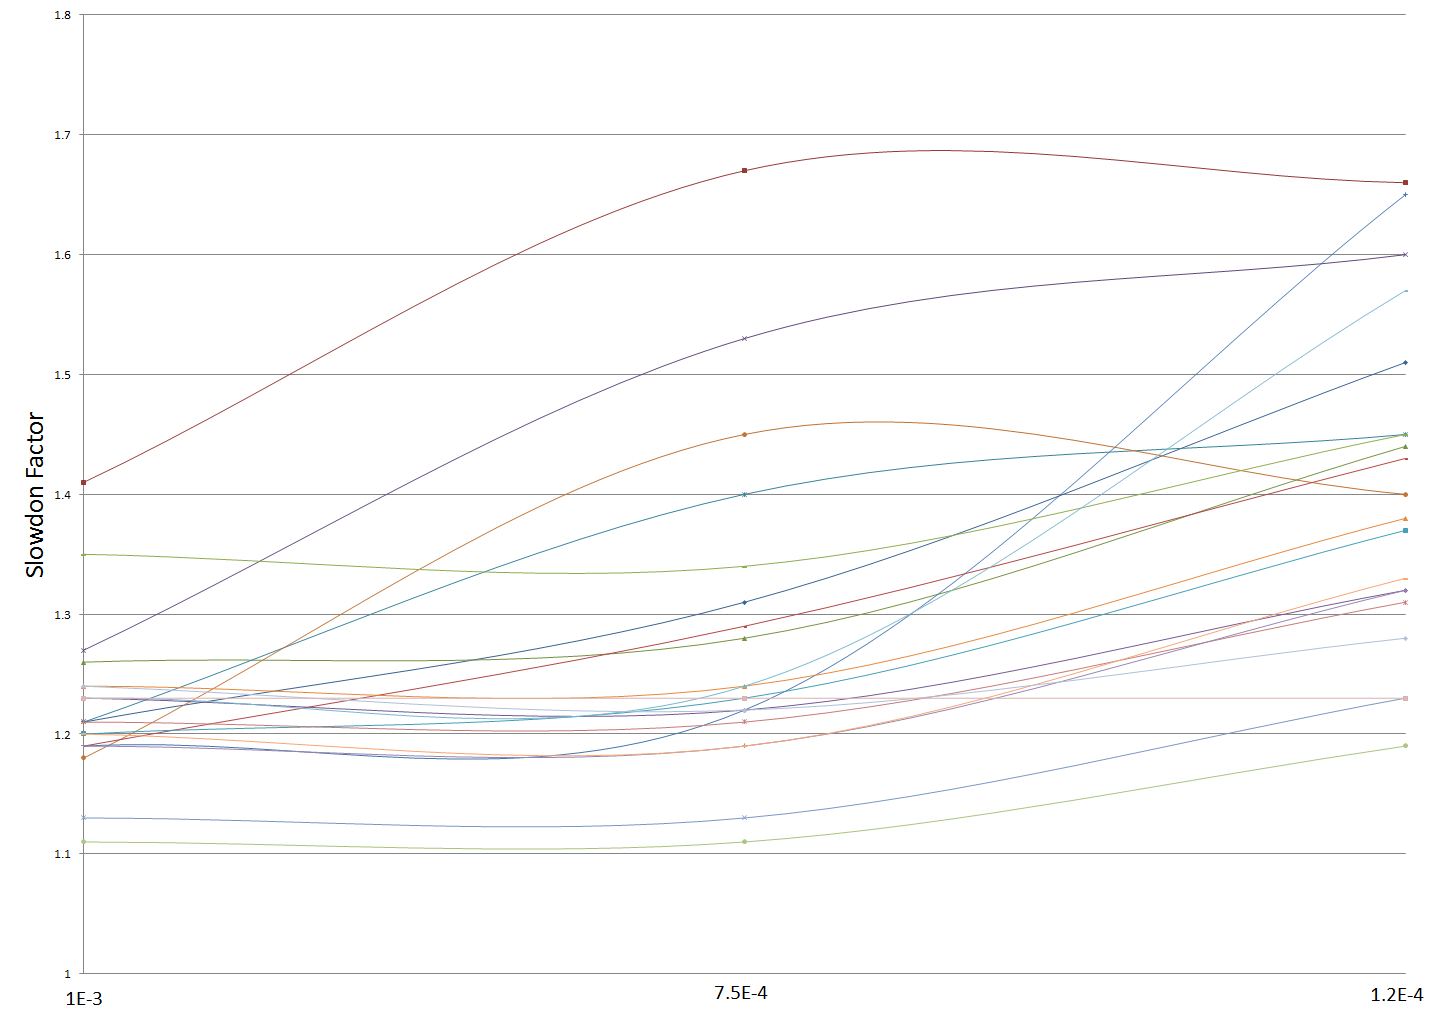
\includegraphics[width=\textwidth]{images/slowdown.png}
         \caption{Slowdown Factors for each Benchmark at Different Recovery Times} \label{slowdownFig} 
      \end{center}


   \end{figure}
   In general, the more partitions the slower the
   resulting circuit, as per Figure \ref{slowdownFig} where each line represents a different circuit. This result is unsurprising, as increasing the number of
   voters increases the number of signals to be routed increasing congestion.
   Mean slowdown is around $1.2\times$--$1.65\times$ depending on target recovery time, though
   it varies considerably from circuit to circuit.
   This compares favourably with \gls{TMR}'ing the entire circuit as a whole, which saw typical slowdowns between $1.1\times$--$1.4\times$
     For our recovery time
   calculations, as they required an estimate of the final circuit clock period
   we used an estimate of $1.8\times$ the original circuit's clock period. As
   we can see from the results, in the general case this factor is quite
   conservative, and we can likely get away with a lower value, say 1.5 for
   most cases.
   


   \section{Running Time}\label{timing}
   
   \begin{table}
      \begin{center}
   \begin{tabular}{lr}
	\toprule
   	Step & Time (s) \\
   	\midrule
   	VPR Original & 225.76\\
   	Partition & 0.56 \\
   	Triplicate & 0.31 \\
   	Join & 0.07 \\
   	Flatten & 0.35 \\
   	Test & 0.92 \\
   	VPR TMR & 5237.50\\
   	\bottomrule
   \end{tabular}
   \caption{Running times for clma with a target recovery time of 2.5e-4s}\label{runningtimes}
   \end{center}\end{table}
   As shown in table \ref{runningtimes}, the largest contributor to the running time in our toolflow is \gls{VPR}, taking several orders of magnitude longer than any other step. Of the time \gls{VPR} took, routing is generally the largest contributor, followed by placement, followed by packing.
   Routing for standard \gls{FPGA} architectures is NP-Complete \cite{npcomplete} with the specific routing algorithm used by \gls{VPR} being $O(k^2\log{k})$ per net on average,
   where k is the number of terminals for the net \cite{VPRBook}.
   


   \section{Recovery Time}
    For the benchmark circuits typical recovery times ranged from $1.2\times10^{-4}$s to $10^{-3}$s. Anything larger is redundant, as the entire circuit fits within one partition, and anything smaller has the circuits unable to be partitioned. The number of partitions and the size of each partition are the two main contributing factors to the recovery time of a partition, therefore the smaller the circuit, the smaller a recovery time its partitions are able to achieve. As the circuit size increases (as measured by the number of \glspl{BLE}) either the size of each partition, or the total number of partitions must increase, driving up the recovery time.
    Table \ref{minrec} details the experimentally determined minimum achievable recovery time for each of the twenty largest \gls{MCNC} benchmark circuits. The estimated final clock period was taken as the mean original clock period for that circuit $\times 1.8$. This value was passed to the partitioner with progressively smaller target recovery times until the partitioner was unable to partition whilst meeting the target recovery time.
    Figure \ref{minrecFig} shows the same information as a scatter plot, making the correlation between circuit size and minimum recovery time more visible.
    
   \begin{table}
   \begin{center}
   \begin{tabularx}{0.8\textwidth}{lRRR}
    Name &  Number of BLEs (original) &  Clock Period (original) (ns) & Minimum Recovery Time ($\times10^{-5}$s)\\
  \midrule
clma & 8365 & 9.21 & 12.2\\
s38584.1 & 6177 & 4.97 & 7.80\\
s38417 & 6042 & 6.27 & 8.50\\
ex1010 & 4598 & 5.92 & 7.30\\
pdc & 4575 & 6.47 & 7.70\\
spla & 3690 & 6.01 & 6.50\\
elliptic & 3602 & 7.72 & 7.60\\
frisc & 3539 & 10.95 & 9.00\\
s298 & 1930 & 8.59 & 6.10\\
apex2 & 1878 & 5.07 & 4.50\\
seq & 1750 & 4.55 & 4.00\\
bigkey & 1699 & 2.28 & 2.80\\
des & 1591 & 3.97 & 3.50\\
alu4 & 1522 & 4.54 & 3.80\\
diffeq & 1494 & 6.58 & 4.80\\
misex3 & 1397 & 4.40 & 3.50\\
dsip & 1362 & 2.24 & 2.60\\
apex4 & 1262 & 4.57 & 3.40\\
ex5p & 1064 & 4.51 & 3.20\\
tseng & 1046 & 5.94 & 3.70\\
   	\bottomrule
   \end{tabularx}
   \caption{Minimum recovery time for circuits}\label{minrec}
   \end{center}\end{table}
      \begin{figure}

      \begin{center}

         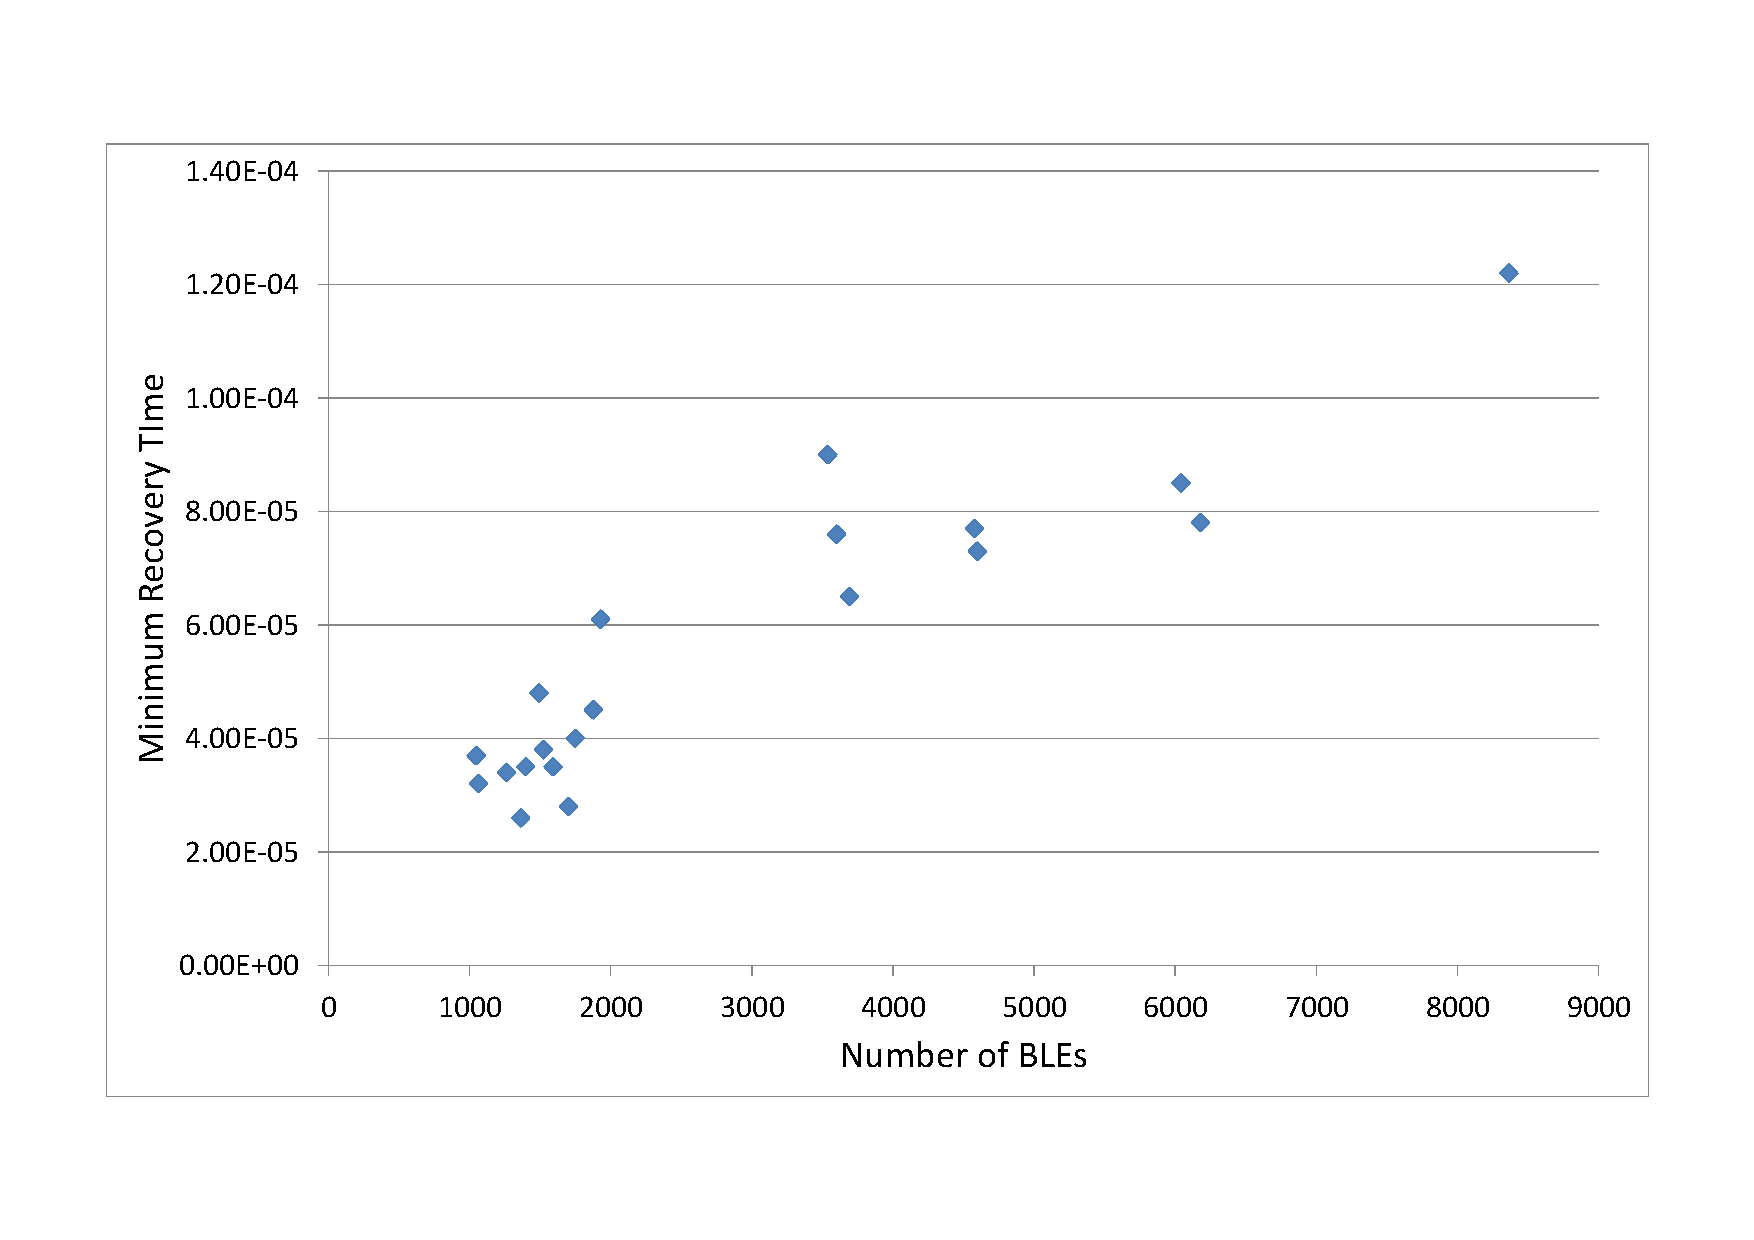
\includegraphics[width=\textwidth]{images/minrec.pdf}
         \caption{Minimum Achievable Recovery Time vs Circuit Size} \label{minrecFig} 
      \end{center}


   \end{figure}


   \section{Depth- vs Breadth-First Traversal}\label{bfs}
   \begin{table}
      \begin{center}
   \begin{tabularx}{\textwidth}{lRRRRRRRRRRR}
   & \multicolumn{2}{r}{Channel Width}&\multicolumn{2}{r}{Network Delay (ns)}&\multicolumn{2}{r}{Logic Delay (ns)}&\multicolumn{2}{r}{Clock Period (ns)}\\
  & Base & TMR & Base & TMR& Base & TMR& Base & TMR\\
  \midrule
Breadth-First & 40 & 58  & 2.37 & 3.53 & 4.16 & 5.53 & 6.52 & 9.06\\
Depth-First & 40 & 54 & 1.96 & 3.53 & 4.16 & 4.51 & 6.11 & 8.04\\
   	\bottomrule
   \end{tabularx}
   \caption{Breadth- vs Depth-first traversals for s38417 with a target recovery time of 2.5e-4s}\label{dvb}
   \end{center}\end{table}
   
   \begin{table}
      \begin{center}
   \begin{tabularx}{\textwidth}{RRRRRRRR}
   Recovery Time ($\times10^{-4}$s)& Number of Outputs & Number of Inputs & Number of cut loops & Number of latches & Number of LUTs & Critical Path Length\\
   \midrule
 2.5 & 723 & 859 & 430 & 714 & 2560 & 17\\
 2.5 & 1029 & 921 & 345 & 565 & 2560 & 9\\
 1.2 & 421 & 606 & 184 & 184 & 976 & 3\\
   	\bottomrule
   \end{tabularx}
   \caption{Breadth-first traversal per partition values for s38417 with a target recovery time of 2.5e-4s}\label{dvbB}
   \end{center}\end{table}
   
   \begin{table}
      \begin{center}
   \begin{tabularx}{\textwidth}{RRRRRRRR}
   Recovery Time ($\times10^{-4}$s)& Number of Outputs & Number of Inputs & Number of cut loops & Number of latches & Number of LUTs & Critical Path Length\\
   \midrule
 2.5 & 775 & 663 & 563 & 567 & 2560 & 30\\
 2.5 & 596 & 683 & 446 & 627 & 2560 & 19\\
 1.2 & 280 & 381 & 150 & 269 & 976 & 10\\
   	\bottomrule
   \end{tabularx}
   \caption{Depth-first traversal per partition values for s38417 with a target recovery time of 2.5e-4s}\label{dvbD}
   \end{center}\end{table}
   
   The values in Tables \ref{dvb}, \ref{dvbB} and \ref{dvbD} are representative samples from a single run. As the partitions generated depend on the estimated clock period which varies from run to run it makes little sense to average per-partition values across runs, especially when the actual number of partitions may vary. As such, while absolute values may change  the general trends hold across all runs.
   
   Using a breadth-first traversal algorithm tends to lead to broader partitions, with correspondingly more inputs and outputs for each partition but shorter critical path lengths.
   Using a depth-first traversal on the other hand leads to deeper but narrower partitions, with fewer inputs and outputs for each partition, but a longer critical path length.
   As each value which is exported from a partition to be used in another needs to be voted on, this means every feedforward or feedback edge requires another \gls{LUT} in the final design.
   As the pipeline depth increases the likelihood of having an internal cycle which needs to be cut increases, so we see more feedback edges, shown by the Cut Loops column in Tables \ref{dvbB} and \ref{dvbD} also leading to more voters. In general however, breadth-first will have more total \glspl{LUT} required. As outlined in Table \ref{dvb}, breadth-first traversal had an extra 1.02ns of logic delay on the critical path from the extra \glspl{LUT}, and required slightly wider routing channels to route the design.
   
   The difference is minor for larger partition sizes, however as the number of partitions increases the effect becomes more pronounced, until with some circuits every almost every single circuit element is voted upon when using a breadth-first traversal, as in Table \ref{dvbbad}.
   Tables \ref{Results1.2e-4DFS} and \ref{Results1.2e-4BFS} in the Appendix list measured slowdowns and area increases for depth- and breadth- first circuits at $1.2\times10^{-4}$.
      \begin{table}
      \begin{center}
   \begin{tabularx}{\textwidth}{RRRRRRRR}
   Recovery Time ($\times10^{-5}$s)& Number of Outputs & Number of Inputs & Number of cut loops & Number of latches & Number of LUTs & Critical Path Length\\
   \midrule
 7.45 & 20 & 1318 & 0 & 0 & 480 & 1 \\
 7.45 & 480 & 1314 & 0 & 0 & 480 & 1 \\
 7.45 & 480 & 986 & 0 & 0 & 480 & 1 \\ 
 7.45 & 480 & 949 & 0 & 0 & 480 & 1\\ 
 7.45 & 480 & 852 & 0 & 0 & 480 & 1\\ 
 7.45 & 480 & 633 & 0 & 0 & 480 & 1\\
 7.45 & 480 & 432 & 0 & 0 & 480 & 1 \\
 7.45 & 480 & 464 & 0 & 0 & 480 & 1 \\
 7.45& 480 & 592 & 0 & 0 & 480 & 1\\
 5.97 & 265 & 135 & 0 & 0 & 278 & 1 \\
   	\bottomrule
   \end{tabularx}
   \caption{Depth-first traversal per partition values for ex1010 with a target recovery time of 7.5e-5s}\label{dvbbad}
   \end{center}\end{table}

   \chapter{Limitations and Future Work}
   Our algorithm implementation is still
   just a first pass at the problem to evaluate its feasibility. There is still
   much work to be done.

   Some notable limitations are that our implementation operates on \gls{BLIF}
   files and targets a theoretical simplified architecture. In practice, it
   would be ideal to use and target industry standard tools, formats and
   architectures.  There are a number of assumptions and approximations made as
   part of the implementation, especially in the calculation of recovery time;
   improving the accuracy of approximations allows the partitioner to find
   better solutions. Additionally, the partitioner itself makes no attempt to
   find an optimal solution; partitions may be closed off before they're full,
   or partitions may be unbalanced with some having many more voters or a much
   longer path length than others.
   There are some straightforward techniques which can be implemented to improve the partitioner, but the limiting factor tends to be the partition size, and when (as in
   the benchmark circuits), there are many more \glspl{LUT} than latches, the
   ability to reduce the number of partitions through clever partitioning is
   extremely limited with most partitions being maximally packed already.
   
   In addition to improving the quality of results, the performance of the algorithm can be easily improved in a few areas.
   The algorithm has a theoretical $O(n^3)$ worst case due to a naive brute force estimation function for the target number of partitions.
   Improving this to not require repartitioning over and over by using more intelligent estimates can reduce the number of passes needed.
   There are a few other sections in the implementation where less than optimal approaches were used though they are likely to provide less dramatic gains.
   Regardless, \gls{VPR} remains the limiting factor, so optimising the partitioner for speed is not especially helpful as it is already significantly faster than \gls{VPR}.
   
   An additional limitation is restrictions on input files.
   The implementation makes some assumptions about the format of input files which, while they hold for all \gls{MCNC} we used, do not necessarily hold for all valid circuits.
   For example, that all latches have the same clock.
   These assumptions will need to be replaced with more robust implementations.


   \chapter{Conclusion}
   This thesis was focussed on developing a new TMR
   partitioning algorithm and assessing the effect of the new \gls{TMR}
   technique on the performance of the twenty largest \gls{MCNC} benchmark circuits. From a performance
   standpoint the algorithm shows promise. While there is still much work to be
   done the initial results collected in this thesis indicate that the
   partitioning method described in Chapter \ref{algorithm} and implemented by this
   thesis is capable of providing more effective fault tolerance with overhead
   not too much greater than typical \gls{TMR} solutions as commonly
   implemented today. Additionally, integrating the algorithm into an existing \gls{CAD} tool flow 
   should be achievable with negligible design time cost, as it requires no to modification to existing code and
   the running time is insignificant compared to that of other steps such as routing.


   \appendix 
   \chapter{Data}
   This appendix tabulates the data used to
   calculate the relationships discussed in this thesis.


   \begin{table}
      \begin{center}
      \footnotesize 
      \begin{adjustwidth}
         {-1cm}{-1.2cm}

         \begin{tabularx}
            {1.1\textwidth}{lRRRRRR}
            \toprule
 Circuit & Number of Partitions &  Number of BLEs (original) &  Increase in BLE Number &  Clock Period (original) (ns) &  Clock Slowdown Factor &  Number of Successful Runs\\
 \midrule
clma & 1 & 8365 & 3.01 & 9.21 & 1.21 & 25\\
s38584.1 & 1 & 6177 & 3.21 & 4.97 & 1.41 & 25\\
s38417 & 1 & 6042 & 3.21 & 6.27 & 1.26 & 25\\
ex1010 & 1 & 4598 & 3.00 & 5.92 & 1.27 & 25\\
pdc & 1 & 4575 & 3.01 & 6.47 & 1.21 & 24\\
spla & 1 & 3690 & 3.01 & 6.01 & 1.18 & 24\\
elliptic & 1 & 3602 & 3.35 & 7.72 & 1.19 & 24\\
frisc & 1 & 3539 & 3.27 & 10.95 & 1.19 & 24\\
s298 & 1 & 1930 & 3.01 & 8.59 & 1.35 & 24\\
apex2 & 1 & 1878 & 3.00 & 5.07 & 1.23 & 24\\
seq & 1 & 1750 & 3.02 & 4.55 & 1.20 & 24\\
bigkey & 1 & 1699 & 3.21 & 2.28 & 1.24 & 24\\
des & 1 & 1591 & 3.15 & 3.97 & 1.13 & 24\\
alu4 & 1 & 1522 & 3.01 & 4.54 & 1.21 & 24\\
diffeq & 1 & 1494 & 3.28 & 6.58 & 1.11 & 24\\
misex3 & 1 & 1397 & 3.01 & 4.40 & 1.19 & 24\\
dsip & 1 & 1362 & 3.17 & 2.24 & 1.23 & 24\\
apex4 & 1 & 1262 & 3.02 & 4.57 & 1.20 & 24\\
ex5p & 1 & 1064 & 3.06 & 4.51 & 1.24 & 24\\
tseng & 1 & 1046 & 3.49 & 5.94 & 1.23 & 24\\
Mean &  &  & 3.13  &  & 1.22 & \\


            \bottomrule 
         \end{tabularx}
         \caption{Results
            for target recovery time $1\times10^{-3}$s} \label{Results1e-3}

      \end{adjustwidth}

   \end{center}\end{table}



   \begin{table}
      \begin{center}
      \footnotesize 
      \begin{adjustwidth}
         {-1cm}{-1.2cm}

         \begin{tabularx}
            {1.1\textwidth}{lRRRRRR}
            \toprule
 Circuit & Number of Partitions &  Number of BLEs (original) &  Increase in BLE Number &  Clock Period (original) (ns) &  Clock Slowdown Factor &  Number of Successful Runs\\
 \midrule
clma & 4 & 8365 & 3.08 & 9.35 & 1.31 & 25\\
s38584.1 & 3 & 6177 & 3.27 & 5.00 & 1.67 & 25\\
s38417 & 3 & 6042 & 3.27 & 6.29 & 1.28 & 25\\
ex1010 & 2 & 4598 & 3.27 & 5.94 & 1.53 & 25\\
pdc & 2 & 4575 & 3.12 & 6.43 & 1.40 & 25\\
spla & 2 & 3690 & 3.12 & 5.89 & 1.45 & 25\\
elliptic & 2 & 3602 & 3.38 & 7.70 & 1.22 & 25\\
frisc & 2 & 3539 & 3.35 & 10.93 & 1.29 & 25\\
s298 & 1 & 1930 & 3.01 & 8.55 & 1.34 & 25\\
apex2 & 1 & 1878 & 3.00 & 5.10 & 1.22 & 25\\
seq & 1 & 1750 & 3.02 & 4.38 & 1.23 & 25\\
bigkey & 1 & 1699 & 3.21 & 2.27 & 1.24 & 25\\
des & 1 & 1591 & 3.15 & 4.02 & 1.13 & 25\\
alu4 & 1 & 1522 & 3.01 & 4.49 & 1.21 & 25\\
diffeq & 1 & 1494 & 3.28 & 6.59 & 1.11 & 25\\
misex3 & 1 & 1397 & 3.01 & 4.50 & 1.19 & 25\\
dsip & 1 & 1362 & 3.17 & 2.23 & 1.24 & 25\\
apex4 & 1 & 1262 & 3.02 & 4.63 & 1.19 & 25\\
ex5p & 1 & 1064 & 3.06 & 4.66 & 1.22 & 25\\
tseng & 1 & 1046 & 3.49 & 5.94 & 1.23 & 25\\
Mean &  &  & 3.16  &  & 1.29 & \\


            \bottomrule 
         \end{tabularx}
         \caption{Results
            for target recovery time $2.5\times10^{-4}$s}
         \label{Results2.5e-4} 
      \end{adjustwidth}

   \end{center}\end{table}

   \begin{table}
      \begin{center}
      \footnotesize 
      \begin{adjustwidth}
         {-1cm}{-1.2cm}

         \begin{tabularx}
            {1.1\textwidth}{lRRRRRR}
            \toprule
 Circuit & Number of Partitions &  Number of BLEs (original) &  Increase in BLE Number &  Clock Period (original) (ns) &  Clock Slowdown Factor &  Number of Successful Runs\\
            \midrule
clma & 14 & 8365 & 3.18 & 8.85 & 1.51 & 3\\
s38584.1 & 6.15 & 6177 & 3.29 & 5.00 & 1.66 & 26\\
s38417 & 7 & 6042 & 3.3 & 6.35 & 1.44 & 26\\
ex1010 & 5 & 4598 & 3.3 & 5.83 & 1.60 & 26\\
pdc & 5 & 4575 & 3.19 & 6.54 & 1.45 & 25\\
spla & 4 & 3690 & 3.17 & 6.01 & 1.40 & 25\\
elliptic & 4 & 3602 & 3.4 & 7.78 & 1.65 & 25\\
frisc & 4 & 3539 & 3.36 & 10.99 & 1.43 & 25\\
s298 & 2 & 1930 & 3.04 & 8.56 & 1.45 & 25\\
apex2 & 2 & 1878 & 3.13 & 5.12 & 1.32 & 25\\
seq & 2 & 1750 & 3.18 & 4.42 & 1.37 & 25\\
bigkey & 2 & 1699 & 3.21 & 2.29 & 1.38 & 25\\
des & 2 & 1591 & 3.23 & 4.00 & 1.23 & 25\\
alu4 & 2 & 1522 & 3.11 & 4.61 & 1.31 & 25\\
diffeq & 2 & 1494 & 3.36 & 6.57 & 1.19 & 25\\
misex3 & 2 & 1397 & 3.12 & 4.47 & 1.32 & 25\\
dsip & 2 & 1362 & 3.31 & 2.25 & 1.57 & 25\\
apex4 & 2 & 1262 & 3.17 & 4.65 & 1.33 & 25\\
ex5p & 1 & 1064 & 3.06 & 4.45 & 1.28 & 25\\
tseng & 1 & 1046 & 3.49 & 5.96 & 1.23 & 25\\
Mean &  &  & 3.23  &  & 1.41 & \\
            \bottomrule 
         \end{tabularx}
         \caption{Results for target recovery time
            $1.2\times10^{-4}$s} \label{Results1.2e-4DFS} 
      \end{adjustwidth}

   \end{center}\end{table}

   \begin{table}
      \begin{center}
      \footnotesize 
      \begin{adjustwidth}
         {-1cm}{-1.2cm}

         \begin{tabularx}
            {1.1\textwidth}{lRRRRRR}
            \toprule
 Circuit & Number of Partitions &  Number of BLEs (original) &  Increase in BLE Number &  Clock Period (original) (ns) &  Clock Slowdown Factor &  Number of Successful Runs\\
 \midrule
clma & \multicolumn{5}{c}{Could not partition for such a small recovery time}&0\\
s38584.1 & \multicolumn{5}{c}{Could not partition for such a small recovery time}&0\\
s38417 & \multicolumn{5}{c}{Could not partition for such a small recovery time}&0\\
ex1010 & 10.23 & 4598 & 3.31 & 5.84 & 1.57 & 22\\
pdc & 12.14 & 4575 & 3.22 & 6.21 & 1.57 & 7\\
spla & 8 & 3690 & 3.19 & 5.97 & 1.49 & 25\\
elliptic & 10.33 & 3602 & 3.42 & 7.54 & 1.66 & 12\\
frisc & \multicolumn{5}{c}{Could not partition for such a small recovery time}&0\\
s298 & 5 & 1930 & 3.05 & 8.43 & 1.50 & 25\\
apex2 & 3 & 1878 & 3.13 & 5.10 & 1.34 & 25\\
seq & 3 & 1750 & 3.21 & 4.44 & 1.40 & 25\\
bigkey & 3 & 1699 & 3.21 & 2.29 & 1.58 & 25\\
des & 3 & 1591 & 3.30 & 3.95 & 1.41 & 25\\
alu4 & 3 & 1522 & 3.14 & 4.53 & 1.32 & 25\\
diffeq & 3 & 1494 & 3.38 & 6.57 & 1.44 & 25\\
misex3 & 3 & 1397 & 3.16 & 4.48 & 1.32 & 25\\
dsip & 3 & 1362 & 3.24 & 2.22 & 1.42 & 25\\
apex4 & 2 & 1262 & 3.26 & 4.63 & 1.40 & 25\\
ex5p & 2 & 1064 & 3.40 & 4.44 & 1.44 & 25\\
tseng & 2 & 1046 & 3.57 & 5.97 & 1.49 & 25\\
Mean &  &  & 3.26  &  & 1.46 & \\

            \bottomrule 

         \end{tabularx}
         \caption{Results for target recovery time
            $7.5\times10^{-5}$s} \label{Results7.5e-5} 
      \end{adjustwidth}

   \end{center}\end{table}


   \begin{table}
      \begin{center}
      \footnotesize 
      \begin{adjustwidth}
         {-1cm}{-1.2cm}

         \begin{tabularx}
            {1.1\textwidth}{lRRRRRR}
            \toprule
 Circuit & Number of Partitions &  Number of BLEs (original) &  Increase in BLE Number &  Clock Period (original) (ns) &  Clock Slowdown Factor &  Number of Successful Runs\\
            \midrule
clma & 14 & 8365 & 3.85 & 8.87 & 1.81 & 1\\
s38584.1 & 6 & 6177 & 3.67 & 4.97 & 1.61 & 15\\
s38417 & 7 & 6042 & 3.59 & 6.29 & 1.62 & 15\\
ex1010 & 5 & 4598 & 3.78 & 5.90 & 1.65 & 15\\
pdc & 5 & 4575 & 3.82 & 6.56 & 1.64 & 15\\
spla & 4 & 3690 & 3.71 & 5.89 & 1.60 & 15\\
elliptic & 4 & 3602 & 3.61 & 7.73 & 1.33 & 15\\
frisc & 4 & 3539 & 3.68 & 10.93 & 1.55 & 15\\
s298 & 2 & 1930 & 3.08 & 8.60 & 1.39 & 15\\
apex2 & 2 & 1878 & 3.39 & 5.09 & 1.43 & 15\\
seq & 2 & 1750 & 3.39 & 4.42 & 1.45 & 15\\
bigkey & 2 & 1699 & 3.35 & 2.28 & 1.63 & 15\\
des & 2 & 1591 & 3.42 & 4.06 & 1.32 & 15\\
alu4 & 2 & 1522 & 3.31 & 4.58 & 1.41 & 15\\
diffeq & 2 & 1494 & 3.38 & 6.50 & 1.39 & 15\\
misex3 & 2 & 1397 & 3.25 & 4.41 & 1.41 & 15\\
dsip & 2 & 1362 & 3.20 & 2.26 & 1.76 & 15\\
apex4 & 2 & 1262 & 3.14 & 4.55 & 1.33 & 15\\
ex5p & 1 & 1064 & 3.06 & 4.61 & 1.21 & 15\\
tseng & 1 & 1046 & 3.49 & 5.92 & 1.22 & 15\\
Mean &  &  & 3.46  &  & 1.49 & \\
\bottomrule

         \end{tabularx}
         \caption{Results for target recovery time
            $1.2\times10^{-4}$s using Breadth- instead of Depth-First Traversal}
         \label{Results1.2e-4BFS} 
      \end{adjustwidth}

   \end{center}\end{table}


   \bibliographystyle{plain} \bibliography{../../../../Bibtex/thesis} %We build
   %with texi2pdf --tidy, so we're really in a build directory several levels
   %away

   \fxfatal{TODO: Change I, we, our, my, etc to passive voice}


\end{document}
